
% !TeX spellcheck = es_ES
\documentclass[11pt,titlepage]{article}
\usepackage{placeins}
\usepackage{comment}

\usepackage[spanish,mexico]{babel}
% !TeX root = informe.tex
\usepackage{alphalph}
\makeatletter
\newcommand*{\fnsymbolsingle}[1]{%
	\ensuremath{%
		\ifcase#1%
		\or *%
		\or \dagger
		\or \ddagger
		\or \mathsection
		\or \mathparagraph
 		\or	\diamond
 		\or	\aleph
% 		\or	\backepsilon %needs amssymb or something
 		\or	\flat
		\else
		\@ctrerr
		\fi
	}%
}
 \newcommand*{\myfnsymbol}[1]{%
 	\myfnsymbolsingle{\value{#1}}%
 }

\makeatother
\newalphalph{\fnsymbolmult}[mult]{\fnsymbolsingle}{}
\renewcommand*{\thefootnote}{%
\fnsymbolmult{\value{footnote}}%
}









%\usepackage{alphalph}
%\makeatletter
% \newcommand*{\myfnsymbolsingle}[1]{%
% 	\ensuremath{%
% 		\ifcase#1% 0
% 		\or % 1
% 		*%   
% 		\or % 2
% 		\dagger
% 		\or % 3  
% 		\ddagger
% 		\or % 4   
% 		\mathsection
% 		\or % 5
% 		\mathparagraph
% 		\or
% 		\diamond
% 		\or
% 		\aleph
% 		\or
% 		\backepsilon
% 		\or
% 		\flat
% 		\else % >= 7
% 		\@ctrerr  
% 		\fi
% 	}%   
% }   
% \makeatother
% 
% \newcommand*{\myfnsymbol}[1]{%
% 	\myfnsymbolsingle{\value{#1}}%
% }
%%  remove upper boundary by multiplying the symbols if needed
%
% \newalphalph{\myfnsymbolmult}[mult]{\myfnsymbolsingle}{}
% \renewcommand*{\thefootnote}{%
% 	\myfnsymbolmult{\value{footnote}}%
% }
\usepackage{graphicx, tikz, subcaption}

\usepackage[onehalfspacing]{setspace}


% HYPERREF
\usepackage{xcolor}
%\definecolor{visigrey}{rgb}{.1,.15,.15}
\definecolor{darkblue}{rgb}{0,0,.6}
\usepackage[
	allcolors=darkblue,%visigrey,
	colorlinks=true,
]{hyperref} %Hyperref antes de geometry!

\usepackage{pdfpages}
\usepackage[a4paper,left=2cm,right=2cm]{geometry}
\geometry{top=1cm,bottom=.5cm}
\savegeometry{titlepage}
\geometry{top=2cm,bottom=2cm}
\savegeometry{main}
\usepackage{pgfplots,tikz,graphicx}
\usepackage{filecontents}
\def\bspace{\(\qquad\qquad\qquad\)}
\usepackage[T1]{fontenc}
\usepackage[utf8]{inputenc}
%\usepackage{sansmathfonts}
\usepackage{lmodern}
%\renewcommand*\familydefault{\sfdefault}
\usepackage[square,numbers,sort]{natbib} % sort=en orden de aparición
\bibliographystyle{unsrtnat}

\setcounter{tocdepth}{2}
% FOOTNOTE
\usepackage{todonotes}
\usepackage{pdfpages}


\def\changemargin#1#2{\list{}{\rightmargin#2\leftmargin#1}\item[]}
\let\endchangemargin=\endlist 
\pgfplotsset{compat=1.16}






\usepackage{listings}
\usepackage{xcolor}

%New colors defined below
\definecolor{codegreen}{rgb}{0,0.6,0}
\definecolor{codegray}{rgb}{0.5,0.5,0.5}
\definecolor{codepurple}{rgb}{0.58,0,0.82}
\definecolor{backcolour}{rgb}{0.95,0.95,0.92}

%Code listing style named "mystyle"
\lstdefinestyle{mystyle}{
  backgroundcolor=\color{backcolour},   commentstyle=\color{codegreen},
  keywordstyle=\color{magenta},
  numberstyle=\tiny\color{codegray},
  stringstyle=\color{codepurple},
  basicstyle=\ttfamily\footnotesize,
  breakatwhitespace=false,         
  breaklines=true,                 
  captionpos=b,                    
  keepspaces=true,                 
  numbers=left,                    
  numbersep=5pt,                  
  showspaces=false,                
  showstringspaces=false,
  showtabs=false,                  
  tabsize=2
}

\lstset{style=mystyle}
\usepackage[scaled=0.85]{FiraMono}
\usepackage{listings}
\usepackage{hyperref}

\lstset{basicstyle = \ttfamily,
        keywordstyle=\bfseries,
        language = Python,
        tabsize=4,
        escapeinside={`}{`}
        }

%\usepackage{bigfoot} % to allow verbatim in footnote
%
% \let\ph\mlplaceholder % shorter macro
% \lstMakeShortInline"

% \renewcommand{\lstlistingname}{Código}
% \renewcommand{\lstlistlistingname }{Códigos \Matlab}
% \lstset{
%   language           =  Python
%   basicstyle         = \mlttfamily,
%   escapechar         = ",
%   mlshowsectionrules = true,
%   numbers = none,
%   tabsize=4,
% }
 % Mostrar codigo python
% GLOSARIO
\usepackage[sort=none,abbreviations]{glossaries-extra}
\setabbreviationstyle{long-short}

% \newabbreviation{fem}
% {FEM}
% {modelo de elementos finitos}


\newglossaryentry{quantumeff}
{
	name=Quantum Efficiency,
	text=quantum efficiency,
	description={Razón de conversión de fotón a electrón para un sensor. Depende de la longitud de onda.}
}

% \newglossaryentry{lst}
% {
% 	name=Linear Strain Triangle,
% 	text=LST,
% 	description={Elemento triangular de 6 nodos. Puede captar gradientes lineales de tensión con precisión arbitraria.}
% }
 
%% DIFFERENTIAL OPERATOR
\makeatletter
\providecommand*{\diff}%
{\@ifnextchar^{\DIfF}{\DIfF^{}}}
\def\DIfF^#1{%
	\mathop{\mathrm{\mathstrut d}}%
	\nolimits^{#1}\gobblespace}
\def\gobblespace{%
	\futurelet\diffarg\opspace}
\def\opspace{%
	\let\DiffSpace\!%
	\ifx\diffarg(%
	\let\DiffSpace\relax
	\else
	\ifx\diffarg[%
	\let\DiffSpace\relax
	\else
	\ifx\diffarg\{%
	\let\DiffSpace\relax
	\fi\fi\fi\DiffSpace}
	

\def\Matlab{\(\textrm{\textsc{Matlab}}\)}%^\textrm{®}

\def\metano{\ensuremath{\mathrm{CH}_4}}
\newcommand{\oxygen}{\ensuremath{\textrm{O}_2}}
\newcommand{\dioxcarb}{\ensuremath{\textrm{CO}_2}}
\newcommand{\dioxsulf}{\ensuremath{\textrm{SO}_2}}
\renewcommand{\d}[1]{\ensuremath{\operatorname{d}\!{#1}}}
\newcommand{\sat}{{\tiny\textrm{sat}}}
\newcommand{\SOx}{\ensuremath{\textrm{SO}_x}}
\newcommand{\NOx}{\ensuremath{\textrm{NO}_x}}

\def\micro{\ensuremath{\mu}}
\def\px{\ensuremath{\mathrm{px}}}
\def\pixrad{\ensuremath{I_{\px}}}
\def\radiance{\ensuremath{I_R}}
\def\radianceunits{\ensuremath{\text{W}\,\text{m}^{-2}\,\text{sr}^{-1}}}
\def\pixradunits{\ensuremath{\text{W}\,\text{m}^{-2}\,\text{sr}^{-1}\,\micro \text{m}^{-1} }}

\def\LEO{\ensuremath{{\mathrm{\tiny LEO}}}}
\def\earth{\ensuremath{\mathrm{tierra}}}
\def\sensor{\ensuremath{{\! \mathrm{\footnotesize sens}}}}



\def\simulationGraphic{
\begin{figure}[htb!]
\centering
\pgfplotsset{colormap/jet}
	\begin{tikzpicture}	
		\begin{axis}[view={30}{40}, width=0.7\textwidth,y dir=reverse,
		title={Radiancia de píxel a 100km de altura},xlabel={Longitud de onda [\micro m]},
		ylabel={Concentración de \metano [ppm]}, zlabel={\pixrad~  [\pixradunits]}]
		\addplot3 [surf, mesh/rows=7, shader=faceted interp]
		table[x=wl, y=ch, z=ir, col sep=comma] {plots/ch4ppmSurf-M7.csv};
		\addplot3 [mesh, black, mesh/rows=7, shader=faceted interp]		table[x=wl, y=ch, z=ir, col sep=comma] {plots/ch4ppmSurf-M7.csv};
		\end{axis}
	\end{tikzpicture}
	\caption{Grafico  de radiancia de píxel en función de longitud de onda y concentración de \metano.}
	\label{fig:ch4IrrVsPpm}
\end{figure}
} % macros para matematica en su mayor parte

% para codigos:

%% CARATULA
\def\colorborde{white} % black or 'white' para que no tenga borde
\def\autor{Ben Romarowski\and Federico Sofio\and Gabriel Torre \and Camila Haene\and Nahuel Letang\and Patricio Whittingslow\and Yann Birnie Scott\and Malena Müller\and Carola Pedrosa\and Gonzalo Reina Kiperman}
%\def\carrera{Open Space}
%\def\empresa{}
\def\fecha{\today}
\def\tema{Space Meters}
\def\titulo{Mapeo de gases de efecto invernadero en la atmósfera por medio de instrumentos de medición de bajo costo}
\def\carrera{}
\def\empresa{}
%% DOCUMENT
\def\resumen{}
\begin{document}
	% Crear y configurar el titulo/caratula del informe
	\pagenumbering{arabic}

\def\headingtype{\bf \small}
\def\openspacelogo{\href{https://www.spaceisopen.com/}{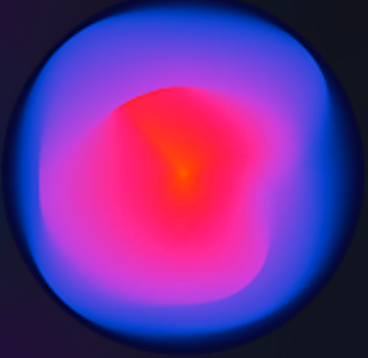
\includegraphics[height=25mm, clip]{caratula/logo}}}

\loadgeometry{titlepage}
\begin{titlepage}
	\centering
	\begin{tikzpicture}[remember picture, overlay]
	\coordinate (top_right) at 
	([xshift=-2.5cm, yshift=-2.5cm]current page.north east);
	\coordinate (top_left) at 
	([xshift=2.3cm, yshift=-2.3cm]current page.north west);
	\coordinate (bottom_right) at 
	([xshift=-1.8cm, yshift=1.8cm]current page.south east);
	\node[inner sep=0, anchor=north west] at (top_left) {};
	\node[yshift = 0.3cm, inner sep=0, anchor=north east] at (top_right) {
	\begin{tabular}{r}
	 {\headingtype \emph{}} \\ [-2pt]
		{\headingtype \carrera} \\[-2pt]
		{\headingtype \emph{\empresa}} \\[-2pt]	
	\end{tabular}
	};
	\draw[double, line width = 0.5pt, color = \colorborde] (top_left) rectangle (bottom_right);
	\end{tikzpicture}\par
	\vfill
	{\centering
		
\includegraphics[width=4cm]{fig/SM.png}\par
	}
	{\Huge \bf  \tema \par}
	\vspace{2.0cm}
	{\LARGE \bf \titulo \par}
	\vspace{2.0cm}
	\begin{tabular}{c}
	\autor~
	\end{tabular}\par
	
	\vspace{1cm}
	
\begin{tabular}{c}
    %  \textbf{Resumen} \\ [10pt]
\end{tabular}\par
\begin{changemargin}{2cm}{2cm} % este comando es personalizado. ver preambulo
{ \resumen\par }
\end{changemargin}\par

	\vspace{2.0cm}
	{\Large \fecha \par}
	\vfill
	\openspacelogo{}
\end{titlepage}
\loadgeometry{main}

 %El siguiente documento tiene la finalidad de plasmar el grado de avance del proyecto haciendo un enfoque en particular en la división de las tareas para llevar a cabo en la etapa de factitibilidad y en detalle de los aspectos más relevantes para el desarrollo del proyecto, en función de esto organizamos equipos de trabajo, para abordar cada una de las tareas.

\newpage
\section*{ }
\section*{Resumen}
En el presente trabajo se muestra el proceso de diseño de un espectrómetro para el análisis de gases de efecto invernadero en la atmósfera terrestre mediante instrumentos de medición de bajo costo. El proyecto será presentado a la competencia de Open-Space organizada por Satellogic.\par

La información obtenida con el espectrómetro será utilizada con fines educativos, quedando los datos bajo libre acceso con licencia \textit{open-source}. Esto permitirá generar interés en otros jóvenes sobre la industria aeroespacial y el \textit{know-how} sobre sistemas espectrales de bajo costo para contribuir a la comunidad open-source con las lecciones aprendidas durante el transcurso del proyecto.

\section*{Agradecimientos}
A Open Space y Satellogic, por organizar la competencia del programa espacial para j\'ovenes que permiti\'o que desarrollemos este m\'odulo satelital.\\\par 

A Satellogic nuevamente, por ser nuestro mentor de proyecto.\\\par 

Al Instituto Tecnológico de Buenos Aires, por ser un lugar donde se nos permite crecer tanto como personas así como profesionalmente, con profesores y personal altamente motivado para enseñar y dar lo mejor con sus alumnos.\\ \par

A Nicolás Mat\'ias Nemirovsky, por estar con nosotros desde el principio del proyecto brindando sus conocimientos técnicos como también organizativos, ayudándonos a mejorar como equipo y como jóvenes profesionales.\\\par

A Horacio Daniel Rinaldi, por ayudarnos con sus amplios conocimientos de la física que logró muy claramente transmitir a sus alumnos a lo largo de los años de su carrera, brindándonos la posibilidad de realizar el presente trabajo y tener la chance de cumplir un sueño. Por mostrarnos lo que es enseñar desde la pasión y no desde la obligación, al día de hoy podemos decir que es nuestro honor y privilegio haber sido sus alumnos.\\\par

A Daniel Andr\'es Jacoby, por orientarnos en el an\'alisis de señales en simulaciones que llevamos a cabo.\\\par

A Miguel Pablo Aguirre, por estar siempre apoyando a sus alumnos a realizar proyectos y actividades extracurriculares.\\\par % falta mas chamuyo

A Dietrich Feist, especialista en el uso de espectroscopía con Transformada de Fourier,  por guiarnos en la relación de especificación técnica a construcción mecánica de un FTIR.


\newpage

\tableofcontents
\newpage


% \pagestyle{fancy}

\section{Introducción}
Actualmente el cambio clim\'atico es el principal problema ambiental global al que se enfrenta la humanidad. Los fenómenos climáticos extremos, la disminución de la calidad del aire y la degradación o enrarecimiento de la capa de ozono estratosférico, entre otros, provocan una pérdida generalizada de biodiversidad. Por este motivo es que el estudio de gases de efecto invernadero en la atmósfera ha tomado importancia en la última década. Hoy en día hay gran interés en lograr una medición de indicadores de contaminación atmosférica a bajo costo. Por lo tanto, este trabajo refleja un gran interés en la obtención de mediciones relevantes de los gases de efecto invernadero de la atmósfera mediante una alternativa coste-efectiva a las opciones comunes espectrales.\\

\subsection{Objetivo}

El objetivo del proyecto consiste en diseñar un sistema innovador coste-efectivo capaz de medir la concentración de gases de efecto invernadero en la atmósfera para la puesta en órbita desde un satélite de la Empresa Satellogic.


\newpage

\section{Planificación del proyecto}

En la siguiente sección se muestran los avances orientados a la organización y conceptualización del proyecto.

\subsection{Arquitectura preliminar del módulo}

El diagrama en bloques que se observa en la Fig.\ref{fig:payload} indica de manera preliminar todos los elemento a tener en cuenta para la realización del módulo para mapeo de gases de efecto invernadero en la atmósfera.


\begin{figure}[htb!]
    \centering
    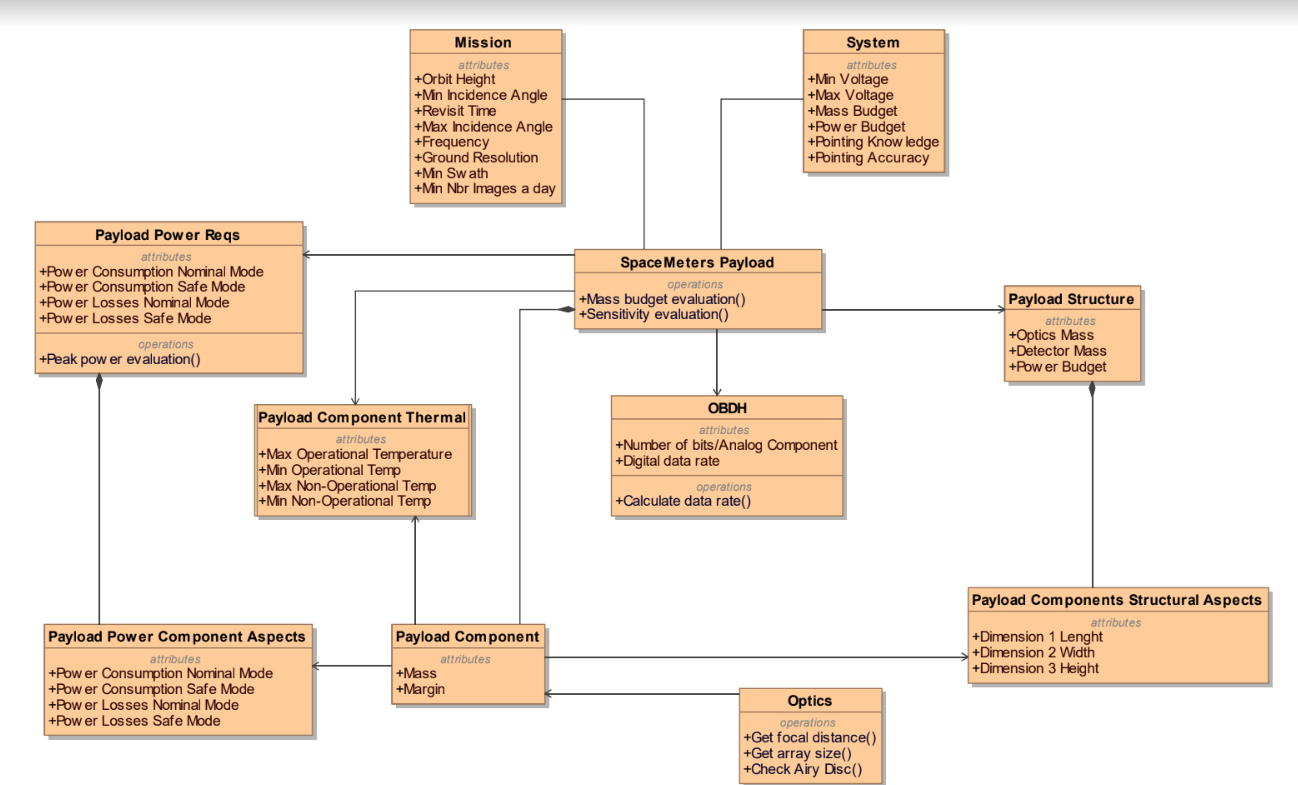
\includegraphics[width=15cm]{fig/payload.png}
    \caption{Diagrama en bloque de la arquitectura del módulo}
    \label{fig:payload}
\end{figure}

\subsection{Análisis de riesgos}

Este análisis resulta de suma importancia a lo largo de todo el proyecto, ya que permite anticiparse a posibles fallas en el momento de diseño, permite ver en qué elementos del proyecto prestar mayor atención y, finalizada cada etapa, permite identificar las lecciones aprendidas.
Para llevar a cabo esto, realizamos un análisis de las posibles problemáticas que se podrían generar durante la realización del proyecto y le asignamos una acción y un responsable para poder resolverla. El modo de cuantificar cada una de las tareas fue asignado un valor en función de la probabilidad de ocurrencia y la severidad de impacto, dando como resultado tres escalas representadas con tres colores diferentes:
%\begin{itemize}
%   \item Verde: Impacto bajo
%    \item Amarillo: Impacto medio
%    \item Rojo: Impacto alto
%\end{itemize}

%\begin{figure}[htb!]
%    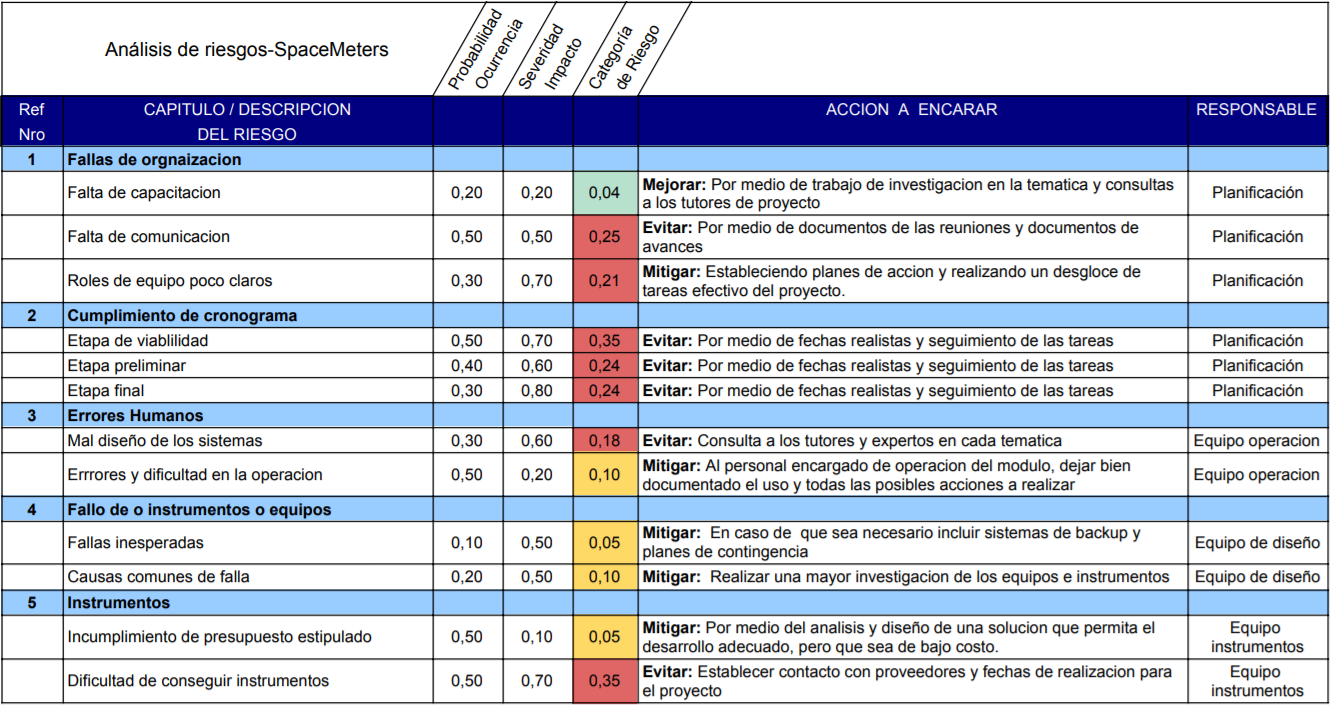
\includegraphics[width=18cm]{fig/riesgos.png}
%    \caption{Análisis de riesgos de proyecto}
%    \label{fig:my_label}
%\end{figure}

%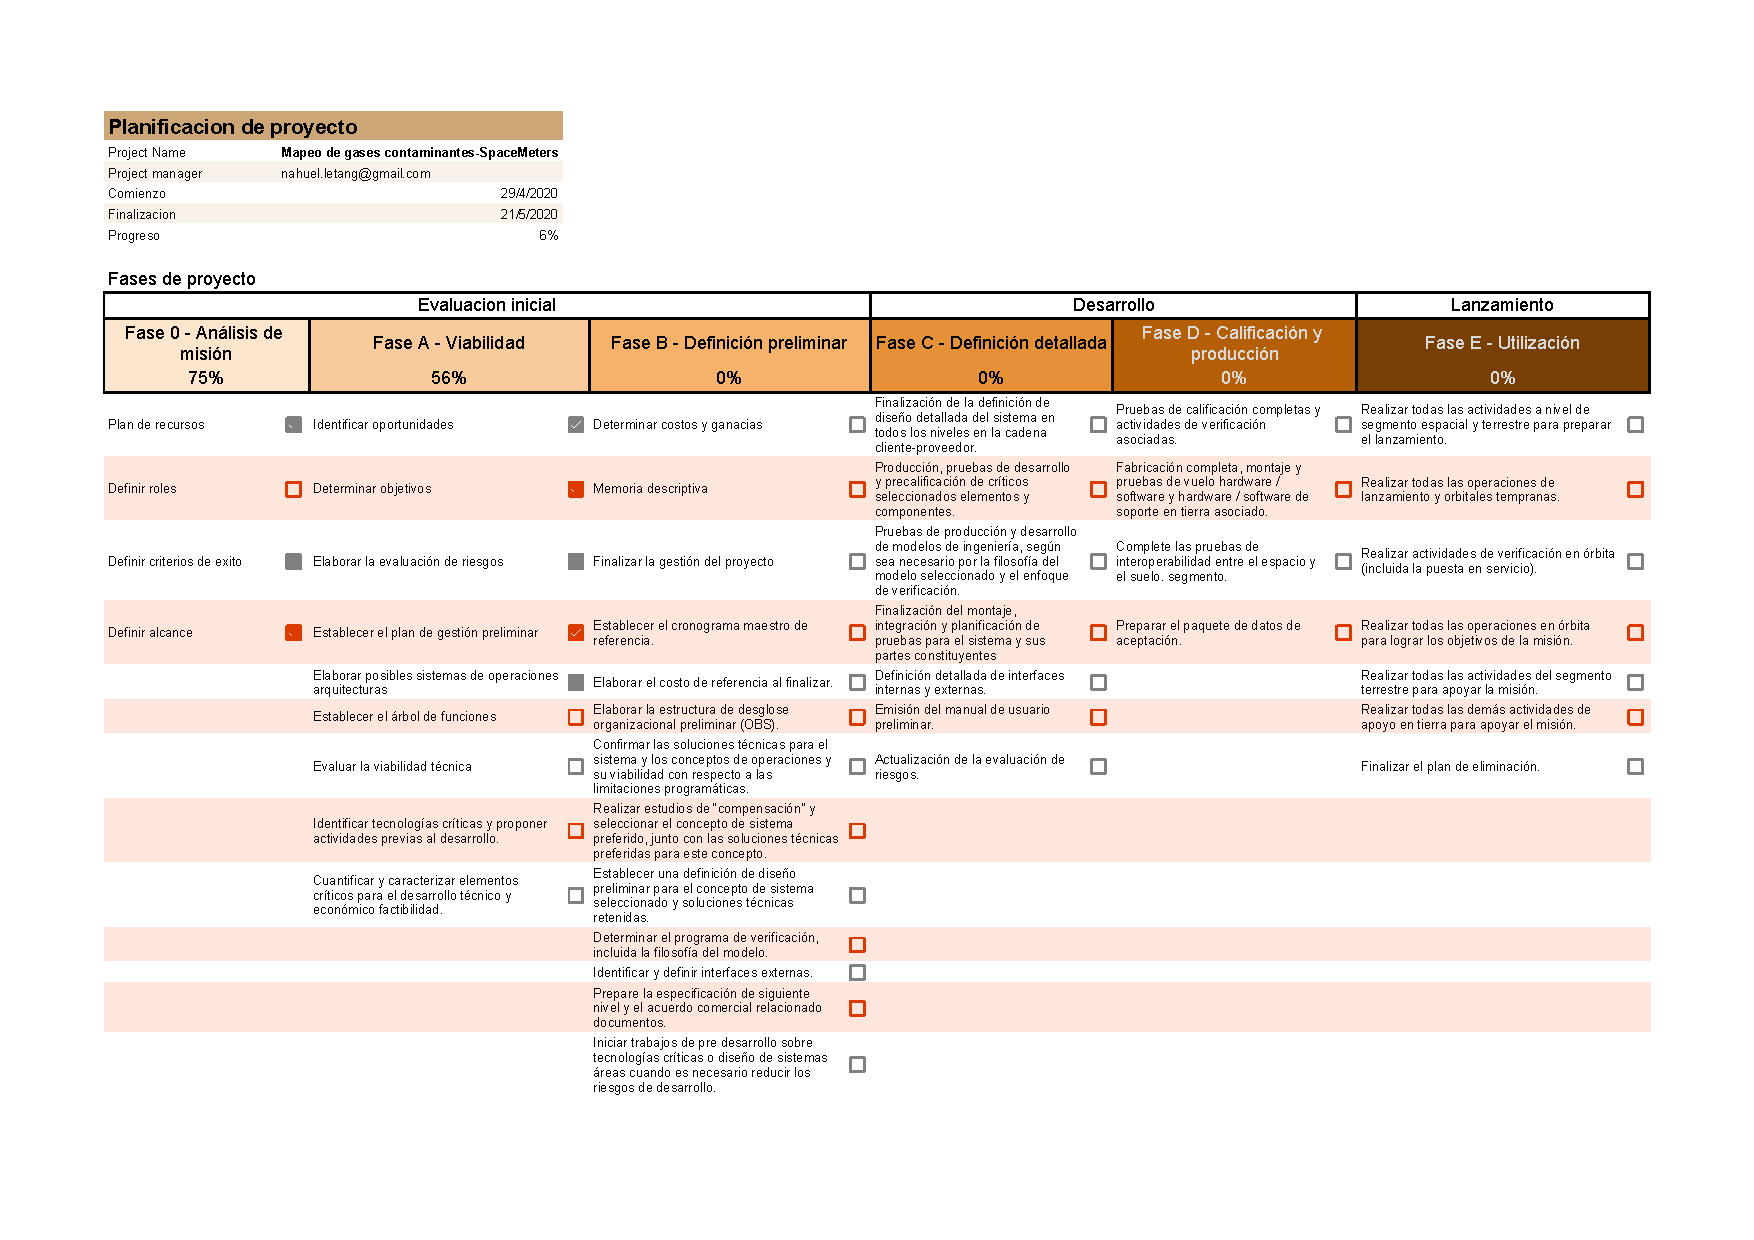
\includepdf[fitpaper, pages={1,2}]{pdf/planificacionProy}
%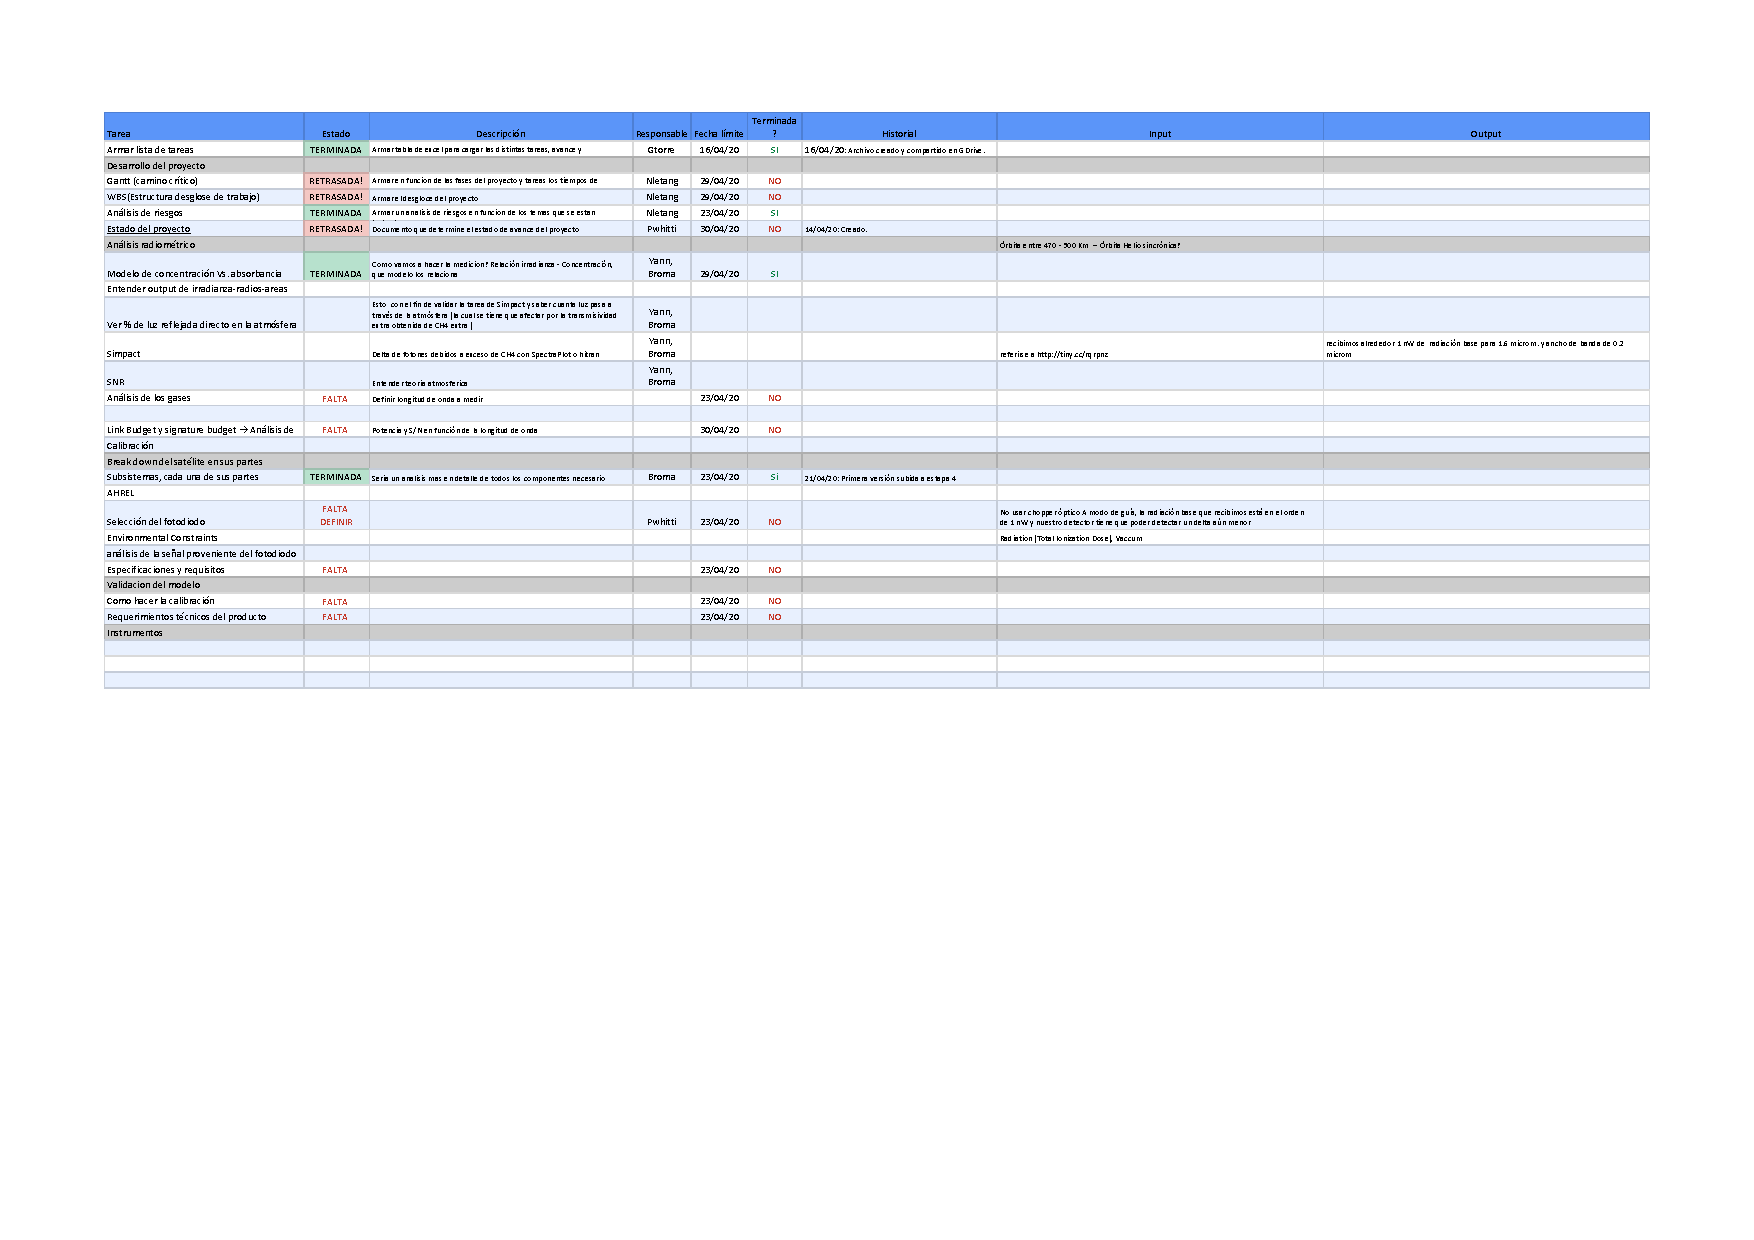
\includepdf[fitpaper]{pdf/tareas}

\newpage

\section{Análisis de gases}

En la presente sección se detallará como se realizó el estudio de gases, desde la selección de gases a estudiar como así también las simulaciones realizadas para el estudio de su concentración en la atmósfera.

\begin{figure}[htb!]
    \centering
    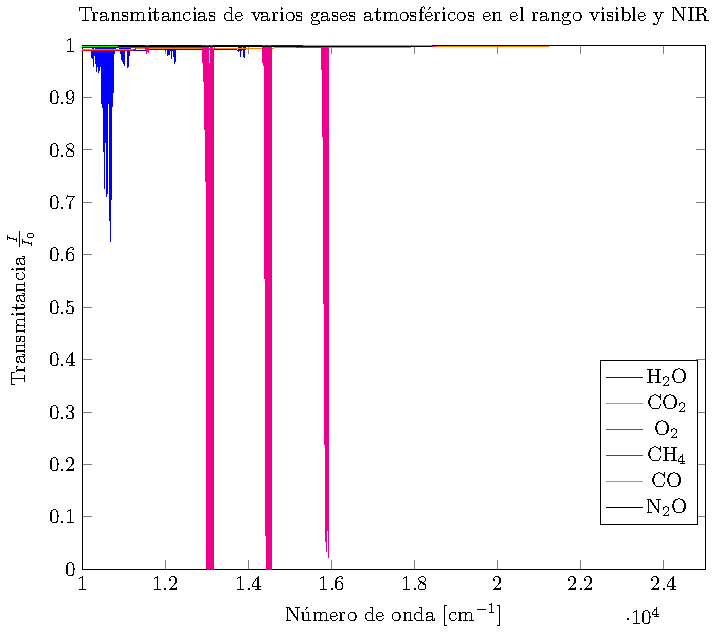
\includegraphics[width=10cm]{pdf/transmitanciaVisibleNIR.pdf}
\end{figure}
\begin{figure}[htb!]
    \centering
    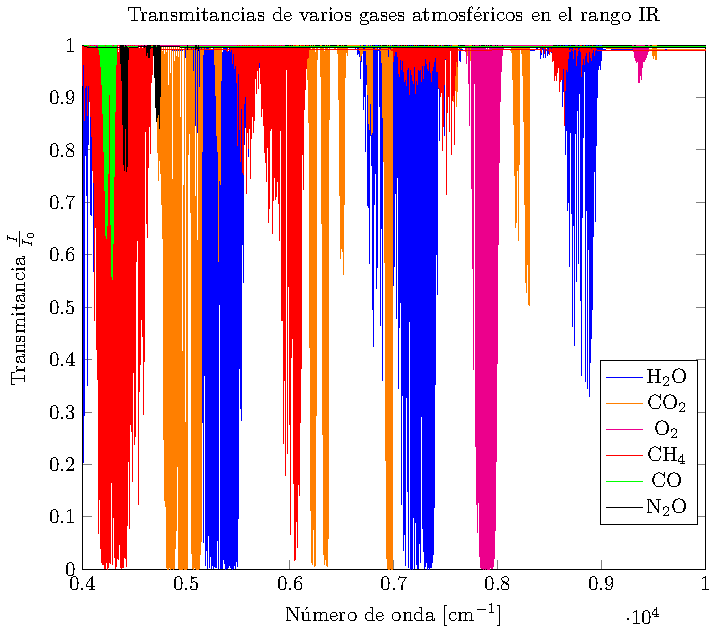
\includegraphics[width=10cm]{pdf/transmitanciaIR.pdf}
    \caption{Datos obtenidos de Spectraplot. Notar que en el número de onda correspondiente a 1,6\micro m 
    ($\approx 6000$cm$^{-1}$) no hay solapamiento entre la absorción del \metano~ y otros gases.}
\end{figure}

\subsection{Selección de indicador}

Para conocer el estado de la atmósfera se necesita monitorear un buen indicador, es decir, una variable ambiental que refleje el estado de algún aspecto del medio ambiente en un momento y espacio determinado. Por ende, el proyecto comienza evaluando los indicadores de la \textbf{Tabla \ref{tab:indicadores}} utilizados en Europa.\par

\begin{table}[htb!]
    \centering
    \begin{tabular}{c|c|c}
        Temas & Indicadores disponibles & Indicadores a medio plazo  \\
        \hline
        \hline
        Cambio clim\'atico & Emisiones de \dioxcarb~ y \metano~& \'Indices de emisi\'on de gases\\
        & & de efecto invernadero\\
        \hline
         & Índices de consumo aparente & \'Indices de consumo aparente \\
        Capa de ozono & de sustancias que agotan & de sustancias que agotan\\
         & la capa de ozono & la capa de ozono e \\
         & & índice total agregado\\
        \hline
        Calidad del aire & Emisiones de \SOx~ y \NOx~ & Exposici\'on de la poblaci\'on \\
        & & a la contaminaci\'on del aire\\
        \hline
         & Intensidad de uso de los & Intensidad de uso de los\\
        Recursos h\'idricos & recursos h\'idricos & recursos h\'idricos \\
        & & y a nivel sustancial\\
        \hline
    \end{tabular}
    \caption{Principales indicadores de la OCDE relacionado con temas climáticos. Ref. \cite{OCDE}}
    \label{tab:indicadores}
\end{table}

Una forma de controlar la emisión de los gases de la \textbf{Tabla \ref{tab:indicadores}}, es teniendo un sensor capaz de medir los fotones que llegan al satélite y comparar la intensidad de cada banda con el espectro de absorción de dichos gases presentes en la atmósfera. \par
El presente trabajo concentra el análisis solamente en el metano. La del mismo varía entre 0.6 y 1.9 ppm dependiendo de la actividad industrial, altura y posición geográfica (figura \ref{fig:atmosphericMethane}).

\begin{figure}[htb!]
    \centering
    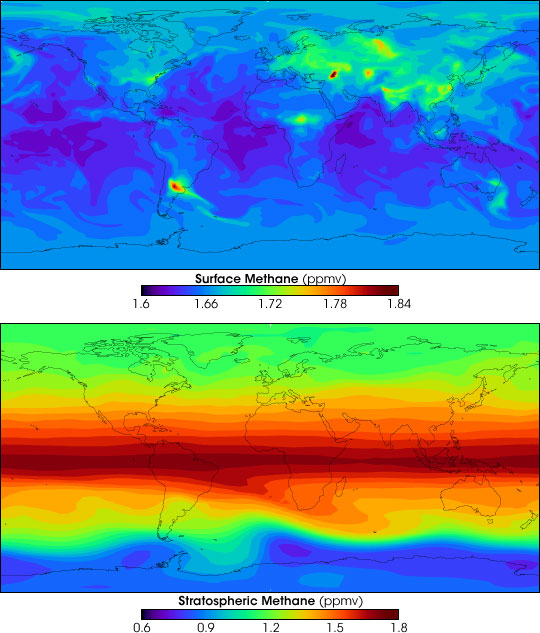
\includegraphics[width=8cm]{fig/AtmosphericMethane.png}
    \caption{Simulaciones mostrando la concentración de metano cerca del suelo y metano estratosférico \cite{hu2018global}.}
    \label{fig:atmosphericMethane}
\end{figure}

\subsection{Descripción Simulación}

Para simular la transferencia radiativa de la atmósfera de la tierra se usó de la librería \texttt{py6s} con Google Colab.
Para utilizar \texttt{py6s} desde el Colab la primera vez, hay que correr el script desde el principio para que se instalen todos los componentes y luego correr el código. La librería tiene perfiles atmosféricos precargados, por lo que solamente se tuvo que cargar el modelo de la atmósfera según nuestro caso.
Con la siguiente función, especificamos las longitudes de onda para un gas determinado:


% \subsection{Curvas de absorción del metano}

A través de la librería mencionada anteriormente se realizó un análisis del espectro de gases en la atmósfera, en donde se hizo particular énfasis en la detección del metano y la influencia de los otros gases a diferentes longitudes de onda, realizado en el siguiente \href{https://drive.google.com/open?id=1dH4wrmwYlQlsIZE5aXH2mcc7xXUcFgpj}{código}. Los resultados (figuras) están en el anexo de figuras (sección \ref{subsec:figuras})

Primero, se analizó la transferencia de metano y se ve que presenta picos de absorción en 1.6, 2,4 y 3.3 µm como se muestra en la Figura \ref{fig:absorbMetano}, donde se puede observar que el valor de intensidad en el pico de absorción se incrementa a medida que aumenta el rango de longitud de onda.

Analizando solamente el pico de los 1.6 µm como se muestra en la Figura \ref{fig:analisis16}, se puede observar que la influencia de los otros gases no es significante, pero tiene la característica que el pico de absorción es el más chico de los tres.

El segundo caso que analizamos fue el del rango de los 2.4 µm. Como se muestra en la Figura \ref{fig:analisis24}, se puede observar que el pico de absorción es mayor que el caso anterior pero la influencia del agua es significativa.


Por último, para el caso del rango de los 3.3 µm, como se muestra en la Figura \ref{fig:analisis33} el pico de absorción es el mayor de todos para el metano, pero si analizamos la influencia del resto de los gases se puede ver que es muy significativa.

Como conclusión, se puede decir que de las tres longitudes de onda estudiadas, la que tiene menor influencia de los otros gases es la de 1.6 µm, pero también se debe analizar si el pico de absorción es lo suficientemente grande para poder ser detectado y, además, se tiene que considerar la influencia del piso de ruido que tengamos en la medición.

\subsection{Comparación con con mediciones de otros satélites}

Un paper escrito por Daniel J. Jacob \href{https://www.atmos-chem-phys.net/16/14371/2016/acp-16-14371-2016.pdf}{de libre acceso} \cite{jacob2016satellite} hace un análisis del modelo teórico que emplean en distintas misiones espaciales para medir metano. La Tabla 1 del mismo especifica la resolución y el rango de longitud de onda empleado para dicho fin. Esto resulta de mucha utilidad para complementar con el análisis del punto anterior, con el objetivo de definir qué rango de longitud de onda es conveniente medir.

%Por lo tanto, se decidió que un punto interesante para seguir trabajando es la misión correspondiente al \href{https://www.spiedigitallibrary.org/conference-proceedings-of-spie/10563/105634O/Fourier-transform-spectrometer-on-GOSAT-and-GOSAT-2/10.1117/12.2304062.full?SSO=1}{GOSAT} (enlace con información interesante sobre los datos constructivos de este satélite).
 
\subsection{Modelo teórico de cómo analizar y medir metano}
Resulta de suma importancia entender la base teórica de lo que se quiere medir para poder seguir avanzando con el análisis.En este documento se hace un mayor énfasis en la base teórica para medir metano en las diferentes misiones, considerando que las técnicas varían en función del rango de longitud de onda que se desea medir.

\subsection{Simulación 6S}
Para obtener una primera aproximación de la influencia de la concentración de metano sobre la radiancia se simuló el siguiente caso:
\begin{itemize}
    \item Diurno, 11hs
    \item Sol cercano al zenit
    \item Vegetación verde. Superficie Lambertiana homogénea
    \item Clima tropical
    \item Altitud de fin de atmósfera 100 km
    \item Rango de longitud de onda estudiado $\lambda \in \{ 1.62, \, 1.70\}$ \micro m
\end{itemize}

Se varió la concentración de metano en la atmósfera entre 0 y 3 ppm en pasos de 0.5 ppm y se obtuvo la superficie mostrada en la figura \ref{fig:ch4IrrVsPpm}.


\begin{figure}[htb!]
\centering
\pgfplotsset{colormap/jet}
	\begin{tikzpicture}	
		\begin{axis}[view={30}{40}, width=0.8\textwidth,y dir=reverse,
		title={Radiancia de píxel a 100km de altura},xlabel={Longitud de onda [\micro m]},
		ylabel={Concentración de \metano [ppm]}, zlabel={\pixrad~  [\pixradunits]}]
		\addplot3 [surf, mesh/rows=7, shader=faceted interp]
		table[x=wl, y=ch, z=ir, col sep=comma] {plots/ch4ppmSurf-M7.csv};
		\addplot3 [mesh, black, mesh/rows=7, shader=faceted interp]		table[x=wl, y=ch, z=ir, col sep=comma] {plots/ch4ppmSurf-M7.csv};
		\end{axis}
	\end{tikzpicture}
	\caption{Grafico  de radiancia de píxel en función de longitud de onda y concentración de \metano.}
	\label{fig:ch4IrrVsPpm}
\end{figure}

\subsection{Simulaci\'on Spectraplot}
Se obtuvieron datos de absorción de luz para una columna de \metano~ utilizando la herramienta Spectraplot \cite{goldenstein2017spectraplot}. Se quiso obtener la absorbancia del \metano~ como lo vé 6S. Las variables de entrada fueron

\begin{itemize}
    \item Longitud de medio $L=100$km. En concordancia con la longitud para la cual integra 6S.
    \item Concentración constante de \metano~ 3 ppm.
    \item Mismo rango de longitud de onda: $\lambda \in \{1.62,\,1.70\}$
    \item Temperatura constante 253K.
    \item Presión constante de 0.35 atm. Es un promedio efectivo de presión ya que la presión no varía linealmente entre 0 y 100 km. \footnote{Cabe destacar que la hipótesis de continuidad deja de ser valida a partir de los 60km y por ende no tiene sentido de hablar de una presión a partir de esta altura. Se podría tomar esto en cuenta para futuros análisis.}
\end{itemize}

con estos datos se obtuvo la transmitancia $T = \frac{I}{I_0}$ (figura \ref{fig:transmitancia100km3ppm}).

\begin{figure}[htb!]
    \centering
	\begin{tikzpicture}
	\begin{axis}[width=0.6\textwidth, title={Transmitancia de una columna de \metano~ de 100km, 3ppm a 0.35atm},xlabel={Longitud de onda [\micro m]},
	ylabel={Transmitancia $\frac{I}{I_0}$}, xmax=1.7,xmin=1.62]
	\addplot[blue] [thick,grid=both]
	table[x=x, y=y, col sep=comma] {plots/trans-3ppm-100km.csv};
	\end{axis}
	\end{tikzpicture}
    \caption{Gráfico obtenido combinando varios resultados del Spectraplot.}
    \label{fig:transmitancia100km3ppm}
\end{figure}



\subsection{Comparaci\'on de resultados entre 6S y Spectraplot}
Se busca comparar los resultados de superponer los efectos de la columna de \metano~ del Spectraplot con los del 6S. Para tal efecto se multiplica la intensidad obtenida del 6S para 0 ppm de \metano~ por la transmitancia obtenida del Spectraplot. Esto resultó en lo que llamaremos una radiancia de píxel modificada. Este perfil de radiancia de píxel fue comparado con la radiancia de píxel obtenida del 6S para 3 ppm haciendo una integración sobre el rango de longitud de onda para obtener la radiancia $\radiance$
\begin{equation}
    \radiance = \int_{\lambda_1}^{\lambda_2} \left.\pixrad(\lambda)\right|_{\text{3ppm}}  \diff \lambda \qquad [\radianceunits] 
\end{equation}
\begin{equation}
    \radiance = \int_{\lambda_1}^{\lambda_2} \left.\pixrad(\lambda)\right|_{\text{0ppm}} \cdot T(\lambda) \diff \lambda \qquad [\radianceunits] \quad \text{Radiancia modificada}
\end{equation}

Los valores obtenidos de radiancia nos dicen el área bajo las curvas de radiancia de píxel. Estos valores son una medida de la potencia que va recibir el sensor. Las radiancias de píxel se muestran en la figura \ref{fig:irradianzasComparativo} y las radiancias integrada se muestran en la tabla \ref{tab:radianciasYModificada}. Se puede observar que la disminución/atenuación de radiancia es del mismo orden de magnitud y difiere poco. La rutina de python que efectuó el cálculo se puede encontrar en \href{https://github.com/spacemeters/radiometry/blob/master/etapa4/validation.py}{github.com/spacemeters/radiometry}.

\begin{table}[htb!]
    \centering
    \begin{tabular}{lcc}
        \textbf{Caso} & \radiance [\radianceunits] & Atenuación [\%] \\ \hline
          \pixrad~ para 0ppm & 1.0858 & Referencia \\
          \pixrad~ para 3ppm & 1.0480 &  3.5\% \\
         \pixrad~ modificada & 1.0339 & 4.8\%
    \end{tabular}
    \caption{Radiancias para dos simulaciones de 6S y una simulación de 6S afectada por la transmitancia obtenida de Spectraplot.}
    \label{tab:radianciasYModificada}
\end{table}




\begin{figure}[htb!]
    \centering
	\begin{tikzpicture}
		\begin{axis}[width=0.8\textwidth, title={Radiancia de pixel vs. longitud de onda}, ylabel={$\pixrad$ [\pixradunits]}, xlabel={Longitud de onda [\micro m]}, xmax=1.7,xmin=1.62]
		\addplot[orange] [grid=both]
		table[x=wl, y=IR, col sep=comma] {plots/modIR-3ppm-100km.csv};
		\addplot[blue,dotted] [ultra thick,grid=both]
		table[x=x, y=y, col sep=comma] {plots/IR0ppm.csv};
		\addplot[red] [thick,grid=both]
		table[x=x, y=y, col sep=comma] {plots/IR3ppm.csv};
		\legend{$\pixrad$ modificada,0ppm,3ppm}
		\end{axis}
	\end{tikzpicture}
    \caption{Resultados de simulación 6S para 0ppm/3ppm y una superposición del caso 0 ppm de 6S con los datos del Spectraplot ($\pixrad$ modificada).}
    \label{fig:irradianzasComparativo}
\end{figure}

	



\subsection{Cálculo de señal recibida}
Una vez obtenida la radiancia de píxel \pixrad~, se calcula la intensidad que llega al sensor según la altura del satélite $h_\LEO$ y el tamaño de píxel $A_\px$, el cual es el área observado sobre la tierra. 

\begin{equation}
    I_\sensor(\lambda) =  \frac{A_\px}{h_\LEO^2} \cdot  \pixrad(\lambda) \qquad [\text{W m}^{-2}\, \micro\text{m}^{-1} ] 
\end{equation}

El sensor \textit{convierte} fotones a electrones. Nos interesa obtener el flujo de fotones sobre la superficie según la longitud de onda. La energía de un fotón es dada por $E_f = \frac{hc}{\lambda}$ 

\begin{equation}
    \Phi_\sensor(\lambda) = \frac{I}{E_f} = \frac{I_\sensor(\lambda) \cdot \lambda }{hc} \qquad [\text{fotones m}^{-2}\, \micro \text{m}^{-1}] 
\end{equation}

Luego, multiplicando el valor $\Phi_\sensor$ por el área del sensor se obtiene la cantidad de fotones que inciden sobre el sensor. Para obtener la cantidad de electrones generados en corriente se integra la expresión obtenida multiplicada por la \gls{quantumeff} $Q$ del sensor, la cual también depende de la longitud de onda del fotón incidente.

\begin{equation}
    n_e = \int_{\lambda_1}^{\lambda_2} A_\sensor \cdot\Phi_\sensor(\lambda) Q(\lambda) \diff \lambda  \qquad [\text{electrones  s}^{-1}]
\end{equation}

La señal obtenida va ser la corriente, dada por
\[
i_\sensor = n_e\cdot q_e = n_e \cdot 1.602176634\times10^{-19} \qquad [\text{Amperes}]
\]
siendo $q_e$ la carga del electrón.
Es necesario aún efectuar el análisis de \textit{signal to noise ratio} (S/N) partiendo del sensor elegido. A continuación se detalla un ejemplo del cálculo que se debería hacer suponiendo algunos valores

\begin{itemize}
    \item Área de sensor $50$mm$^2$
    \item Área de pixel observado de 100km$^2$ (área de Manhattan)
    \item Variación de 1\% de la potencia recibida, que podría corresponder a una variación de 1ppm de \metano~ en la atmósfera según la tabla \ref{tab:radianciasYModificada}
    \item Quantum efficiency igual a 50\% constante
\end{itemize}

\[
\Delta i_\sensor = \Delta n_e \cdot q_e = \frac{A_\sensor A_\px \cdot q_e}{h c  h_\LEO^2 } \cdot \int_{1,62}^{1.70} \lambda \cdot\Delta \pixrad(\lambda) Q(\lambda) \diff \lambda = 8.5363\times 10^{-8} \text{A}
\]
La corriente correspondiente a una variación del 1\% de \metano~ sería
\begin{equation}
    \Delta i_{sens}= 1\% i_{sens}= 8.5363\times 10^{-10} \text{A}
\end{equation}

En base a este resultado creemos que para poder medir metano primero se tendría que comprobar un módulo preliminar. El objetivo de este módulo preliminar sería comprobar la idea detrás de un FTS y obtener un espectro de la tierra antes de intentar medir una intensidad del orden del nano-ampere.


%La pregunta es contundente ¿como medimos esta corriente?
%Formas de aumentar $\Delta i_\sensor$:
%\begin{itemize}
%    \item Acercarse lo más posible al rango de longitudes de onda donde el CH4 tiene más influencia (entre 1.665 y 1.6675)
%    \item Aumentar $A_\px$, tener en cuenta la distancia focal.
%    \item Aumentar $A_\sensor$, limitado por espacio disponible y lentes.
%    \item Cambiar el modo de vibración observado a alguno que presente mayor absorbancia.
%\end{itemize}{}

\begin{comment}


\section[Instrumentos]{Instrumentos de sensado de radiación}\label{sec:instrumentos}
Para poder lograr el objetivo planteado, se necesita de un instrumento capaz de captar un rango de longitudes de onda de interés y la radiancia de la misma. Existen varios instrumentos capaces, a continuación se presentan los mas relevantes durante el estudio del presente trabajo.
  
\subsection{Hiper-espectrómetro}
Estos instrumentos permiten obtener imágenes hiper-espectrales, es decir, imágenes que tienen información sobre las distintas longitudes de onda que componen cada uno de los píxeles de la imagen obtenida. Estos equipos requieren un sistema óptico complejo \cite{zou2017design} para poder separar la luz incidente en cada una de sus componentes y poder formar una imagen para cada una de ellas. Este sistema suele ser costoso pero de alta resolución. Sin embargo, en caso de que la aplicación del hiper-espectrómetro sea viable, es posible hacer un estudio de dos gases de efecto invernadero: el \dioxcarb~ y el \metano. De acuerdo con la Fig. \ref{fig:espectro}, para el \dioxcarb~ las longitudes de onda más favorable a analizar se encuentran entre 1.60mm y 2.00mm ya que las líneas de absorción se encuentran lejos de la de otros gases, por lo que es más fácil distinguirlas. Esta cualidad es muy importante ya que es probable que nuestro instrumento de medición tenga baja resolución. Para el metano \metano~, las longitudes de onda favorables se encuentran alrededor de 1.65 y 2.33mm.

\begin{figure*}[ht!]
    \centering
    \begin{subfigure}[t]{0.45\textwidth}
        \centering
        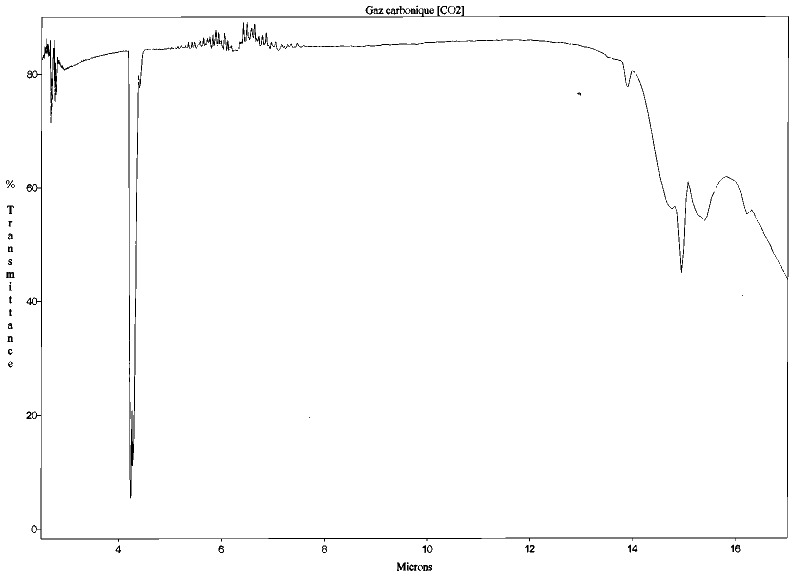
\includegraphics[height=60mm]{fig/CO2.jpg}
        \caption{\dioxcarb~}
        \label{fig:CO2}
    \end{subfigure}%
    ~ 
    \begin{subfigure}[t]{0.45\textwidth}
        \centering
        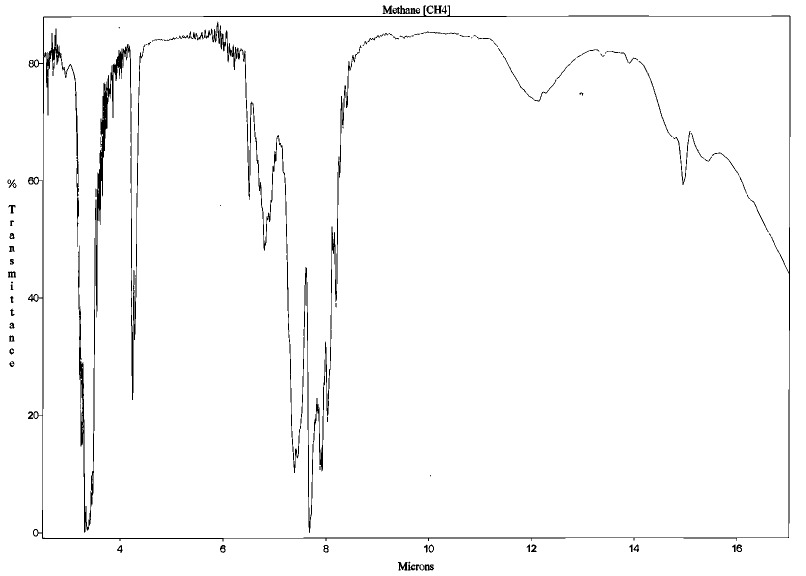
\includegraphics[height=60mm]{fig/CH4.jpg}
        \caption{\metano~}
        \label{fig:CH4}
    \end{subfigure}
    \caption{Espectros de absorción, Ref. \cite{GAZ}.}
    \label{fig:espectro}
\end{figure*}

    \subsection{Espectrómetro}
    En caso de no poder aplicar un hiper-espectrómetro, evaluaremos la posibilidad de aplicar un espectrómetro. Este posee el mismo sistema de funcionamiento, pero un rango de frecuencias acotadas entre el infrarrojo, visible y ultra-violeta. Los mismos suelen ser de construcción simple y menos costosos. En caso de utilizar un espectrómetro, podemos medir emisiones de \dioxsulf, el dióxido de azufre es liberado a la atmósfera debido a actividades humanas y naturales tal como uso de combustibles fósiles o erupciones volcánicas. El mismo es 
    causante de lluvia ácida, lo cual acidifica océanos y elimina bosques de coníferas. Siguiendo el trabajo de la universidad de Heildelberg Ref. \cite{espectrometro}, es posible medir el espectro de absorción del \dioxsulf~ que se observa en la Fig. \ref{fig:SO2}. Con esta opción se debería lidiar con la superposición de algunas de las bandas del ozono de igual forma que lo realiza el instrumento GOME Ref. \cite{espectrometro}.
    
    \begin{figure}[ht!]
    \centering
    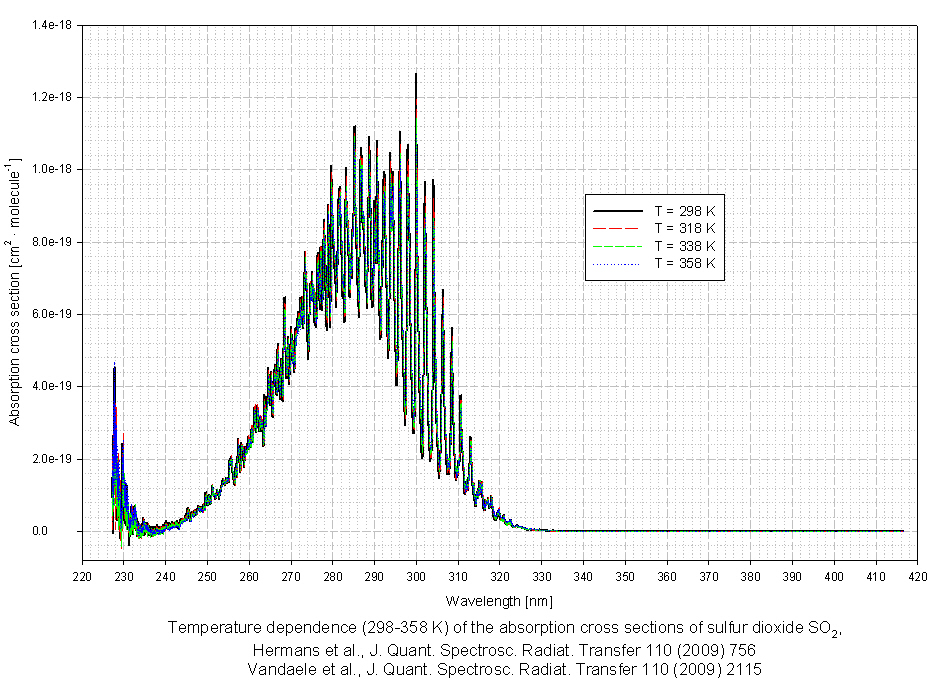
\includegraphics[width=0.8\textwidth]{fig/SO2_2.jpg}
    \caption{Espectro de absorción ultravioleta del \dioxsulf, Ref. \cite{SO2}.}
    \label{fig:SO2}
\end{figure} 

    %Consiste en una cámara donde se descompone la luz entrante y se obtiene la intensidad de las longitudes de onda. Suelen ser de construcción simple y baratos pero su rango de funcionamiento es acotado debido a los sensores de luz y la red de difracción.

    \subsection{Radiómetro}
Es un instrumento que sirve para medir las intensidades de las radiaciones de longitudes de onda bien definidas. Existen varios tipos de radiómetros que en general difieren en la forma de medición que emplean. Una explicación más detallada se encuentra en \nameref{sec:teoria_radiometria}. Si bien aún hace falta hacer un estudio exhaustivo de aplicabilidad de todos los instrumentos planteados, este sensor fue explicado con más detalle ya que en este estudio preliminar de los costos y robustez mecánica, es uno de los instrumentos más viables para el proyecto. La principal diferencia en la utilización del mismo es que el instrumento mide en un rango de frecuencias mucho más limitado en comparación con los espectrómetros, por lo que se suelen colocar varios radiómetros en conjunto para así cubrir un rango de interés. A diferencia del principio óptico de funcionamiento de los espectrómetros, el radiómetro funciona detectando radiación electromagnética mediante una antena. Por ejemplo: En la Fig.\ref{fig:MHSchan} se observa c\'omo con los canales 3, 4 y 5 se mapea un pico de absorción del vapor de agua.\par
Entonces, basándonos en este concepto es posible elegir alguna de las frecuencias de absorción de alguno de los gases de interés planteados, de forma tal que dicha frecuencia se encuentre alejada de modos de vibración de los demás gases presentes en la atmósfera. A su vez será necesario desarrollar un sistema para filtrar el ruido \cite{johnson2016cubesatRadiometer} ya que hoy en día hay mucha interferencia humana en las frecuencias inferiores a 40GHz.
    
    \begin{figure}[htb!]
    \centering
    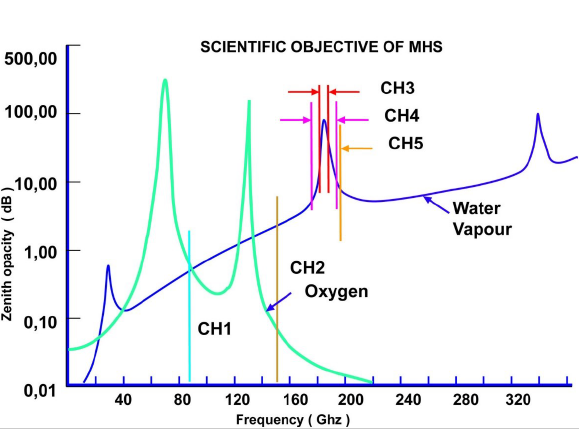
\includegraphics[width=0.6\textwidth]{fig/MHS-channels.png}
    \caption{Vista de canales del radiómetro a bordo de la misión MHS y las curvas de absorción (opacidad) del ox\'igeno y vapor de agua.}
    \label{fig:MHSchan}
    \begin{itemize}
    \item 89GHz: canal para información de temperatura y emisividad superficial de la tierra y detecta precipitación de baja altura. ($\lambda_{89G} = 3.36$mm)
    \item 157GHz y 183GHz: para información de humedad atmosférica. ($\lambda_{157G} = 1.91$mm y $\lambda_{183G} = 1.64$mm)
\end{itemize}
\end{figure}
    
    %Por ejemplo, los que funcionan midiendo las diferencias de temperatura se denominan "detectores térmicos". Un ejemplo de este tipo de radiómetro es la termocupla, que produce una diferencia de potencial cuando se incrementa la temperatura. Otro tipo de radiómetro es el que funciona con lo que se conoce comúnmente como "detectores cuánticos", como por ejemplo la placa fotográfica Becquerel.\cite{radiometro}. 

\subsection{Espectro-radiómetro}
Un espectro-radiómetro es usado para mediar la radiación espectral usando varios rangos espectrales. Posee un sistema de medición óptica, que permite medir luz desde 380nm a 780nm aproximadamente. Este instrumento es ideal para utilizarse en lugares donde se necesitan mediciones precisas tomadas bajo condiciones reales.\cite{espectroradiometro}
    
Según los estudios de mercado realizados, cuanta más resolución tiene el instrumento, más costoso se vuelve. Por eso, de los cuatro instrumentos previamente mencionados, el hiper-espectrómetro resulta ser el más costoso.

\end{comment}



\section{Misiones Espaciales estudiadas}
En la presente sección se mencionan las principales misiones espaciales estudiadas cuyo objetivo es la medición remota de gases en la atmósfera mediante un satélite, es decir que tienen un objetivo similar al buscado en este trabajo.

\subsection{GOSAT (Greenhouse Gases Observing Satellite) }

La primera misión espacial estudiada es la del satélite \textbf{GOSAT} cuyo objetivo consiste en medir la concentración de los principales gases de efecto invernadero del espacio (\dioxcarb~ y \metano).\par
Esta misión es un proyecto conjunto de la Agencia de Exploración Aeroespacial de Japón (JAXA), el Instituto Nacional de Estudios Ambientales de Japón (NIES) y el Ministerio del Medio Ambiente de Japón (MOE).\par

El GOSAT fue el primer satélite de observación terrestre dedicado a medir en forma regular los gases de efecto invernadero en la atmósfera terrestre y fue lanzado el 23 de enero de 2009.


\subsubsection{Instrumentos de medición}

El GOSAT utiliza dos instrumentos de medición. El sensor de infrarrojo cercano y térmico para el espectrómetro de transformada de Fourier de observación de carbono (\textbf{TANSO-FTS} de sus siglas en inglés) detecta los espectros de absorción de gas del infrarrojo de onda corta solar (\textbf{SWIR}) reflejado en la superficie de la tierra, así como el infrarrojo térmico (\textbf{TIR)} irradiado desde el suelo y la atmósfera. El TANSO Cloud and Aerosol Imager (\textbf{TANSO-CAI}) es un radiómetro ultravioleta (UV), visible, infrarrojo cercano y SWIR diseñado para determinar sondeos claros de las mediciones TANSO-FTS y para proporcionar propiedades ópticas de nubes y aerosoles.\cite{MissionGOSAT}.

    \begin{figure}[htb!]
    \centering
    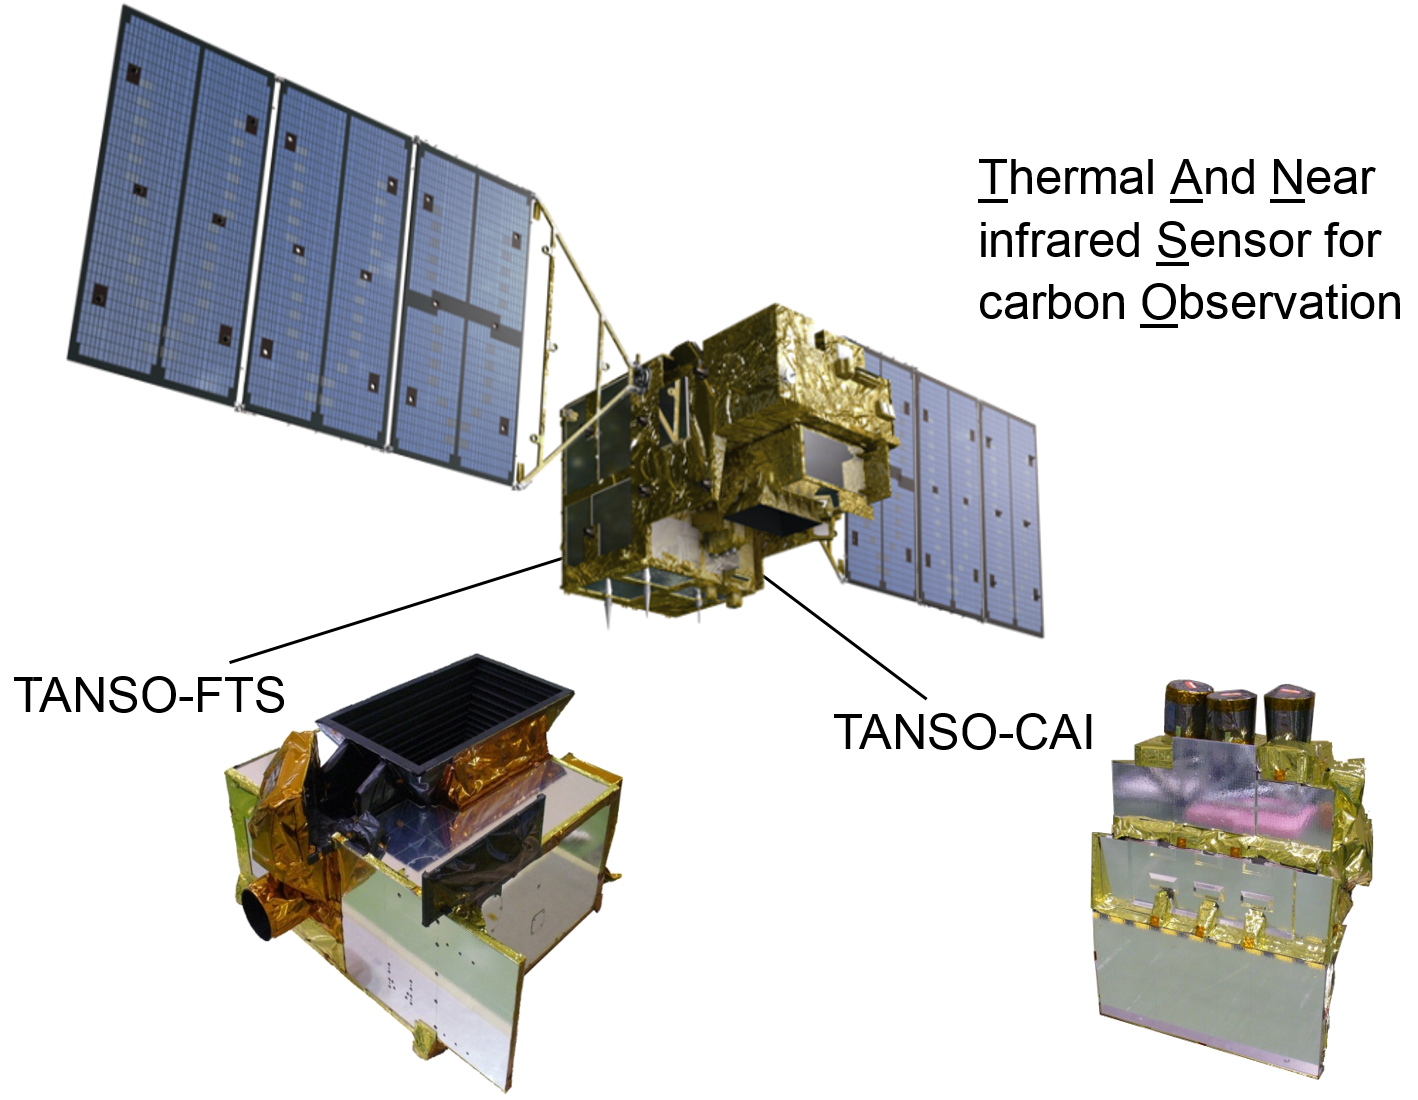
\includegraphics[width=0.6\textwidth]{fig/GOSAT-TANSO.png}
    \caption{Fotos del TANSO-FTS, CAI y vista de diseño del satélite GOSAT en órbita. Ref. \cite{MissionGOSAT}.}
    \label{fig:GOSAT-TANSO}
\end{figure}


\subsubsection{TANSO-FTS}

El instrumento \textbf{TANSO-FTS} mide la radiancia espectral reflejada de la superficie terrestre. Mediante espectrometría por Transformada de Fourier puede medir la concentración de gases presentes en la atmósfera.\par
Los gases que estudia el \textbf{TANSO-FTS} son \oxygen~,\dioxcarb~ y \metano. La concentración de \oxygen~  se obtiene de la región de líneas de absorción correspondientes a 1.6 µm, en las cuales las intensidades son menos dependientes de la temperatura. La región de 2.0 µm puede usarse para la obtención de concentración de \dioxcarb. El \metano~ también se obtiene de la región de 1.6 µm.\par
Para el caso de \oxygen~ también se utiliza una banda de 0.76 µm para estimar la longitud efectiva de la trayectoria óptica, que es un parámetro clave para la recuperación de la densidad de la columna. Como la concentración de \oxygen~ es constante, bien conocida y distribuida uniformemente en toda la atmósfera, esto permite usarla como referencia. 

    \begin{figure}[htb!]
    \centering
    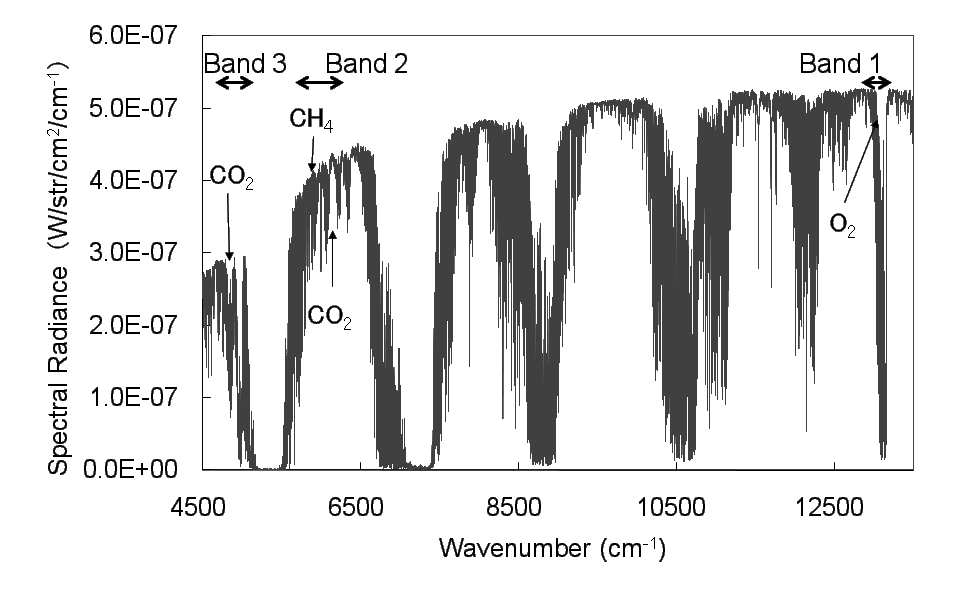
\includegraphics[width=0.65\textwidth]{fig/GosatSimulatedSpectra.png}
    \caption{Cobertura espectral simulada para el TANSO-FTS en la región SWIR. Ref. \cite{FTS-GOSAT}.}
    \label{fig:GosatSimulatedSpectra}
\end{figure}

\subsubsection{TANSO-CAI}

El \textbf{TANSO-CAI} es un radiómetro utilizado para medir nubes y características de aerosoles para mejorar la precisión de los datos del \textbf{TANSO-FTS}. La longitud de onda central se determina a partir del análisis de un momento. Este instrumento tiene una cobertura espacial continua, un campo de visión más amplio y una resolución espacial más alta que el \textbf{TANSO-FTS}, lo cual permite detectar la distribución espacial de nubes y aerosoles.\cite{CAI-GOSAT}

\subsection{MERLIN (Methane Remote Sensing Lidar Mission)}

Esta es una misión franco-alemana que busca poner en órbita a partir de 2023 un satélite capaz de medir \metano~ con una precisión sin precedentes para una misión de estas características. Si bien es una misión aun en desarrollo, entender su principio de medición puede ser de utilidad para el desarrollo del proyecto.\par
MERLIN se instalará en el bus satelital \textit{Myriade Evolutions}, el cúal fue desarrollado por CNES en conjunto a la industria espacial francesa.\par
La carga útil del satélite, es un LiDAR activo que puede medir a través de nubes delgadas y durante la noche. La misma esta siendo desarrollada por la Administración Espacial DLR en Alemania.

    \begin{figure}[htb!]
    \centering
    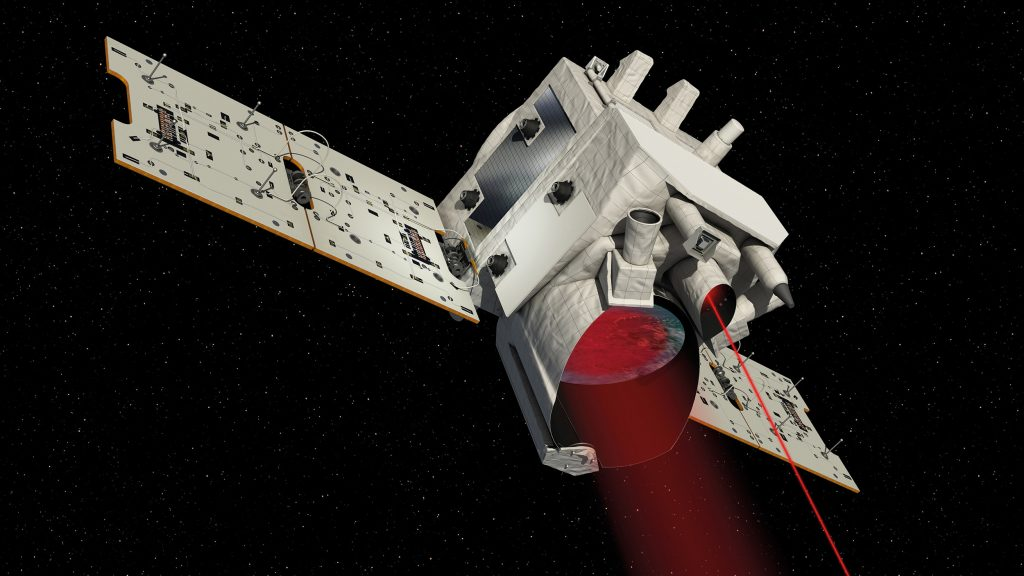
\includegraphics[width=0.6\textwidth]{fig/MERLIN.jpg}
    \caption{Representación del satélite MERLIN en órbita. Ref. \cite{MERLIN}.}
    \label{fig:MERLIN}
\end{figure}

\subsubsection{Principio de Funcionamiento}

El Lidar de metano incluye un láser capaz de emitir luz en dos longitudes de onda diferentes, permitiendo realizar mediciones muy precisas de la concentración de metano en todas las latitudes, independientemente de la luz solar. Las longitudes de onda están en el rango infrarrojo y se eligen para que una sea absorbida por el metano, mientras que la otra no. El satélite envía dos pulsos simultáneamente al mismo lugar en el suelo y luego los captura y registra los pulsos reflejados con un telescopio.
La presencia de metano en la atmósfera debilita solamente a uno de los pulsos. Esta diferencia permite a los científicos determinar la cantidad de metano entre el satélite y la superficie de la Tierra.

\section{Selección del Instrumento de sensado}

Posterior a la investigación sobre instrumentos de sensado de radiación, misiones espaciales de sensado remoto de gases e intercambios con especialistas en el área, se decide utilizar como instrumento de sensado un Espectrómetro por Transformada de Fourier (\textbf{FTS} de sus siglas en inglés). La elección de un FTS como instrumento de sensado para el proyecto se decidió debido a que permite obtener información sobre varias frecuencias de la radiación incidente y por el éxito del mismo en misiones como lo es la misión GOSAT.

\subsection{FTS: Principio de Funcionamiento y Medición}

Un Espectrómetro por transformada de Fourier se podría decir que es similar a un Interferómetro de Michelson, sin embargo tiene pequeñas diferencias y un objetivo distinto.\par
La principal diferencia entre este Espectrómetro y el Interferómetro es que el primero reemplaza la pantalla donde se ve el Patrón de interferencia por un fotodetector, también se necesita que un espejo permita generar una diferencia de camino óptico. Esto se puede lograr moviendo el espejo linealmente. En la \textbf{Figura \ref{fig:Michelson}} se puede observar un esquema de intererómetro de Michelson, mientras que en la \textbf{Figura \ref{fig:FTS}} se puede observar el esquema de un FTS.\par

    \begin{figure}[htb!]
    \centering
    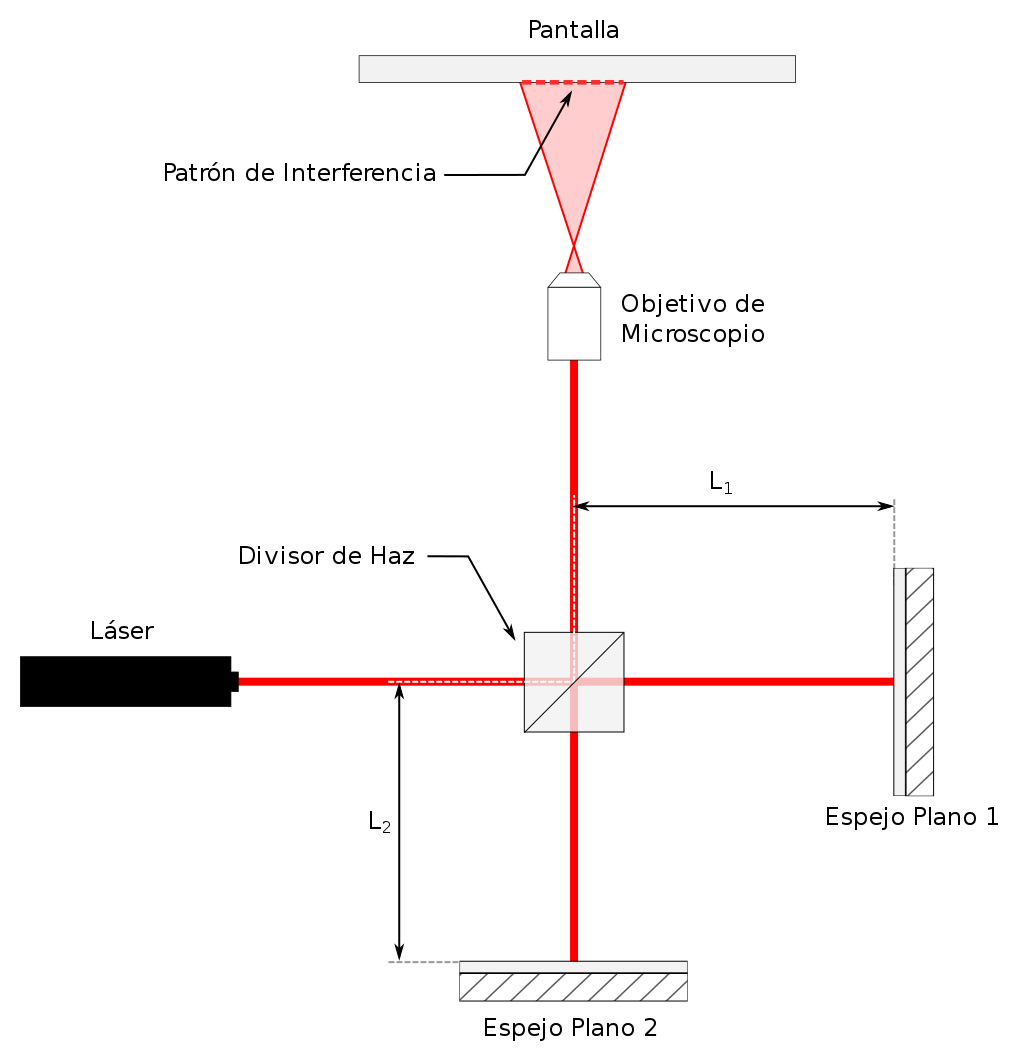
\includegraphics[width=0.6\textwidth]{fig/interferometroMichelson.png}
    \caption{Esquema de un Interferómetro de Michelson. Ref. \cite{Michelson}}
    \label{fig:Michelson}
\end{figure}

    \begin{figure}[ht!]
    \centering
    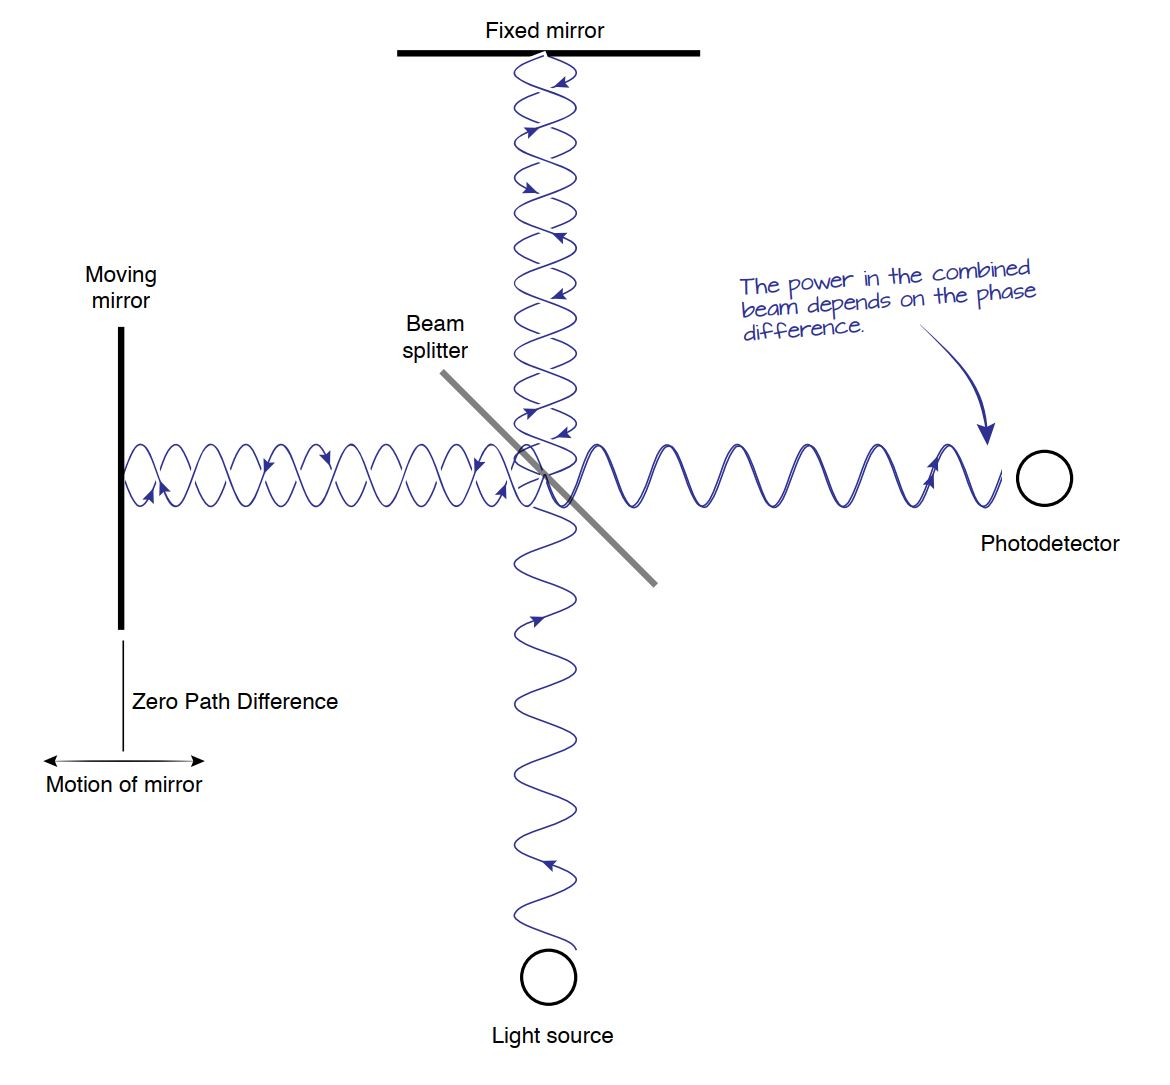
\includegraphics[width=0.6\textwidth]{fig/FTS.jpg}
    \caption{Esquema de un FTS. Ref. \cite{FTS}.}
    \label{fig:FTS}
\end{figure}

El principio de funcionamiento se explicará para el caso de una fuente de luz monocromática.\par
A medida que se mueve el espejo, va cambiando la diferencia de camino óptico entre los haces, lo cual genera máximos y mínimos por interferencia constructiva como también destructiva. Esto implica un haz, a la salida del divisor, que depende directamente de la diferencia de camino óptico, lo cual se traduce en una señal periódica (idealmente) en el fotodetector.\par
    \begin{figure}[ht!]
    \centering
    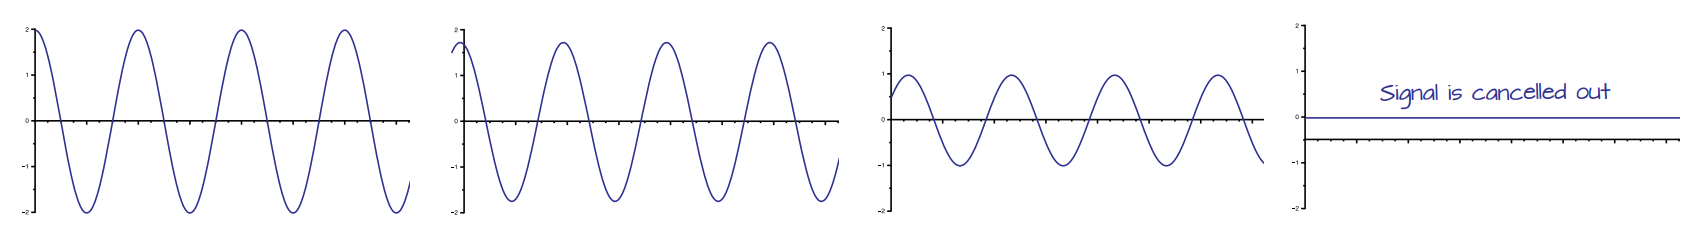
\includegraphics[width=0.9\textwidth]{fig/FTSmaxmin.png}
    \caption{Amplitud del haz en función de la distancia. Ref. \cite{FTS}.}
    \label{fig:InterfFTS}

\end{figure}

Cuando llega el haz al fotodetector, esto se traduce en una señal que va desde un valor máximo a un mínimo. El máximo es en un punto de interferencia constructiva, con una diferencia de camino óptico múltiplo de la longitud de onda y el mínimo en un punto de interferencia destructiva, con una diferencia de camino óptico de la mitad de la longitud de onda.\par
El fotodetector tiene una tasa de muestreo determinada y es por este motivo que debe moverse el espejo con una resolución pequeña y de forma precisa, para muestrear la señal en distintos puntos con distintas diferencias de camino óptico para reproducir la señal exitosamente.

    \begin{figure}[ht!]
    \centering
    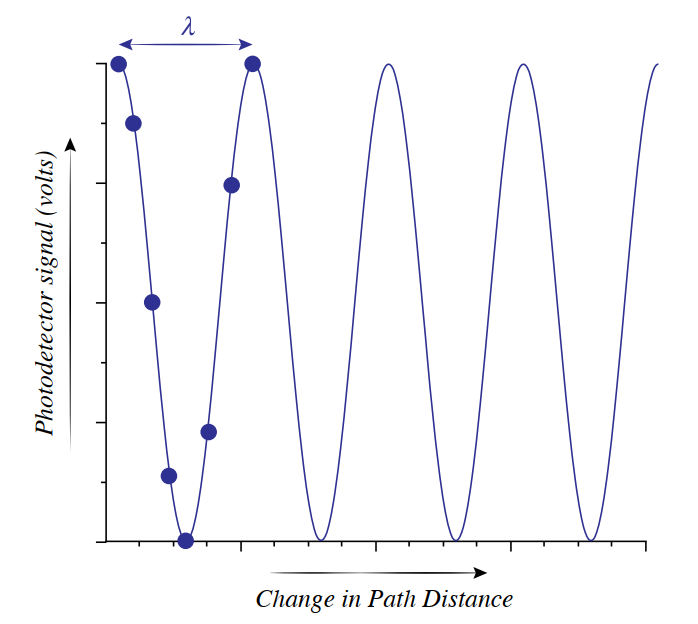
\includegraphics[width=0.5\textwidth]{fig/Measure FTS.png}
    \caption{Señal en el fotodetector. Ref. \cite{FTS}.}
    \label{fig:MeasureFTS}
\end{figure}

De esta manera se obtiene con un interferómetro de Michelson una señal eléctrica con la misma longitud de onda que la de la fuente lumínica. Si a esta señal se le aplica una transformada de Fourier se puede obtener un interferograma donde se encuentran todas las frecuencias de la señal. Al ser la fuente lumínica de luz monocromática, la única frecuencia observable en el interferograma será la de la fuente lumínica.\par

Todo el análisis anterior es válido para una fuente lumínica con varias longitudes de onda presentes. Es decir, que mediante este método se puede obtener una señal eléctrica que contenga toda la información de las frecuencias en la fuente lumínica de manera \textit{codificada}. \par
A continuación se muestra un ejemplo simulado donde la señal que llega al fotodetector contiene las frecuencias de 1 a 30, en la \textbf{Figura \ref{fig:FTS-SIM1}} se puede observar el resultado que se obtendría al transformar la señal.\par

\FloatBarrier
    \begin{figure}[ht!]
    \centering
    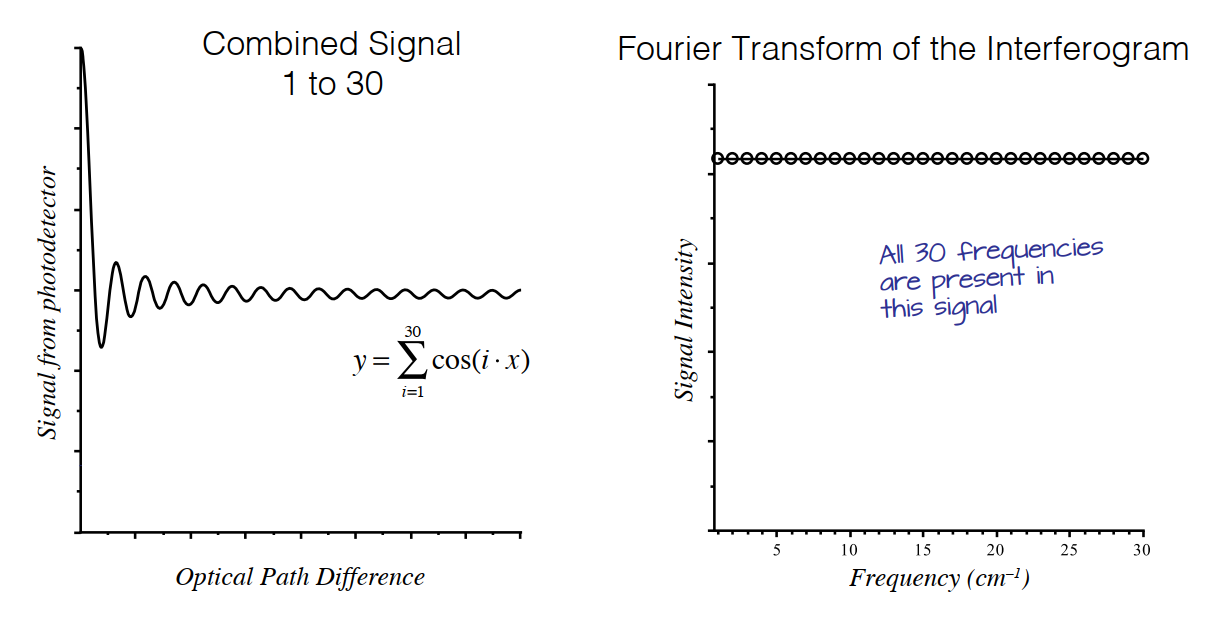
\includegraphics[width=0.7\textwidth]{fig/FTS-SIM1.png}
    \caption{Señal y Transformada para un caso multifrecuencias. Ref. \cite{FTS}.}
    \label{fig:FTS-SIM1}
\end{figure}

Para el caso anterior pero simulando con la ausencia de la frecuencia correspondiente a 10, se obtiene un interferograma donde se observa justamente que dicha frecuencia no esta presente. Dicho resultado se puede observar en \textbf{Figura \ref{fig:FTS-SIM2}}.\par
\FloatBarrier
    \begin{figure}[ht!]
    \centering
    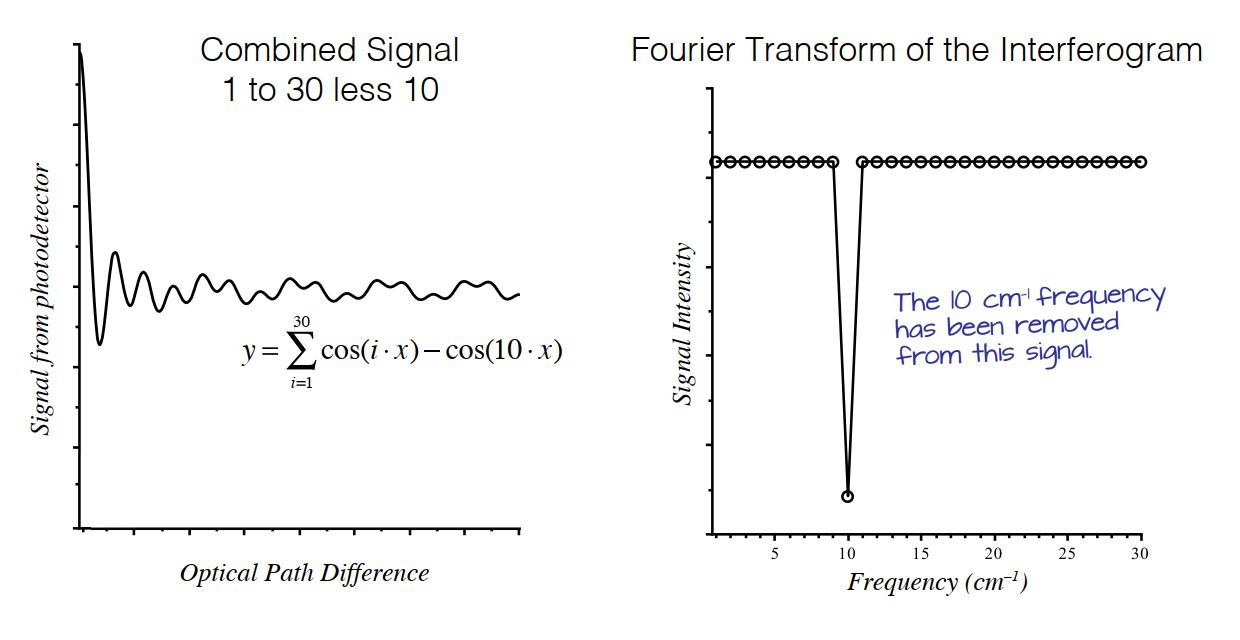
\includegraphics[width=0.7\textwidth]{fig/FTS-SIM2.png}
    \caption{Señal y Transformada para otro caso multifrecuencias. Ref. \cite{FTS}.}
    \label{fig:FTS-SIM2}
\end{figure}

Sin embargo para una medición real, entran en consideración otros efectos como la transmitancia y el impacto de la tasa de muestreo, por lo que un gráfico real sería algo diferente.\par
Para un caso considerando transmitancia no se tendría valores booleanos (presencia y ausencia de frecuencia), sino que el gráfico representaría valores intermedios, como se puede observar en la \textbf{Figura \ref{fig:FTS-SIM3}}. %Mientras que un gráfico de una medición real tiene una forma parecida al de la \textbf{Figura \ref{fig:espectro}}.

    \begin{figure}[ht!]
    \centering
    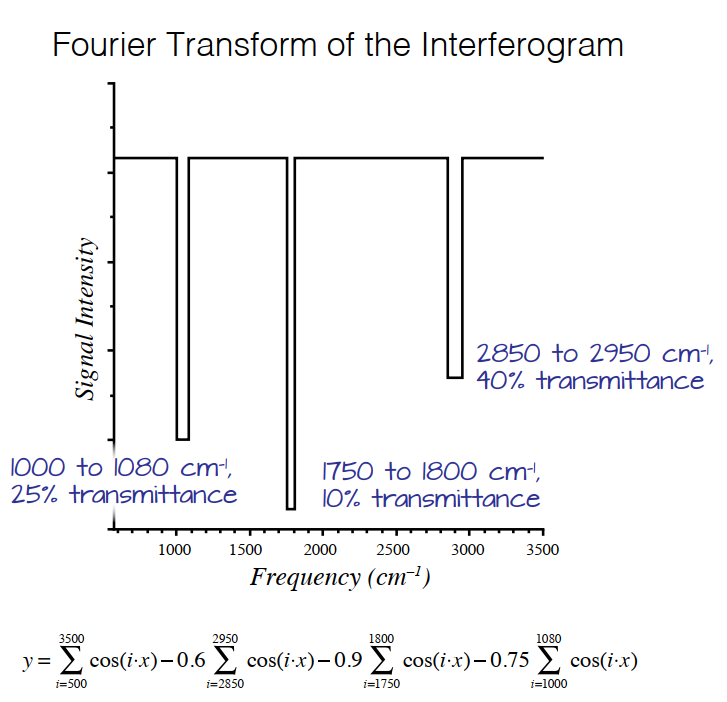
\includegraphics[width=0.55\textwidth]{fig/FTS-SIM3.png}
    \caption{Transformada para un caso considerando transmitancia. Ref. \cite{FTS}.}
    \label{fig:FTS-SIM3}
\end{figure}



\subsection{Consideraciones de Especialistas}

Este proyecto busca medir gases de efecto invernadero, por lo que el rango de medición del espectrómetro será el infrarrojo. Es decir, mediremos los gases mediante espectroscopía infrarroja por transformada de Fourier o \textbf{FTIR} de sus siglas en inglés.\par

Debido al gran nivel técnico que requiere la medición por espectroscopía infrarroja y aún más en el espacio, se decidió contactar con personalidades de la industria aeroespacial como también con agencias espaciales, para que nos guíen con consideraciones a tener en cuenta en el desarrollo de nuestro proyecto. Principalmente se destacan las comunicaciones con dos personalidades:
\begin{itemize}
    \item Dr. Guillermo Rozas de la \textbf{CNAE} (Comisión Nacional de Energía Atómica) quién trabaja en Espectroscopia.
    \item Dr. Dietrich Feist de la \textbf{DLR} (Centro Aeroespacial Alemán) quién trabajó en el proyecto MERLIN y en el centro de investigación de gases de efecto invernadero de DLR.
\end{itemize}
\par

Durante el intercambio de mensajes con el Dr. Rozas, se comentó sobre los cuidados que deben tenerse durante la construcción del mecanismo de espejo móvil. Dicho mecanismo tiene suma importancia ya que la resolución en un FTIR es
inversamente proporcional a la diferencia de camino óptico máxima, además de que se debe pasar por la condición de caminos ópticos iguales (en inglés Zero Path Difference) para interpretar el cero de las mediciones.\par
Para lograr el movimiento del espejo se pensaron dos alternativas. La primera mover el espejo mediante un piezoeléctrico. El Dr. Rozas comento que es una solución de buena estabilidad y velocidad, pero con baja resolución. Para solucionar esto se necesita un piezoeléctrico muy grande.\par
La segunda alternativa es mover el espejo linealmente, mediante una reducción con engranajes acopladas a un servomotor. Con esta solución se obtiene buena resolución pero es mecánicamente más frágil y susceptible a tener variaciones de velocidad.\par

La distancia entre puntos sampleados a lo largo del camino del espejo, define la longitud de onda mínima que se puede medir, ya que son inversamente proporcionales.
El Dr. Rozas nos comentó que para que estos datos se puedan interpretar correctamente, se debe conocer la posición del espejo en dichos puntos con muy buena precisión, como mínimo media longitud de onda de lo que se busca medir
e idealmente un cuarto.\par
También nos comentó que pueden haber señales espúreas superpuestas, si la fuente de luz tiene longitudes de onda menores al límite mínimo definido por el sampleo (frecuencia de Nyquist). Sin embargo esto se puede evitar utilizando un filtro pasa-largo.\par

Con el Dr. Dietrich Feist se realizó una videollamada para atender nuestras dudas sobre la tecnología FTS y la viabilidad de utilizarla en un satélite. Él nos comentó acerca de su trabajo en el proyecto MERLIN y varias consideraciones que hay que tener en cuenta para una misión de estas características.\par
Durante la llamada se pudieron obtener conclusiones y comentarios de gran utilidad. En primer lugar se debe tener mucho cuidado con el armado de la unidad óptica, debido a que los espejos pueden desalinearse debido a vibraciones. Lo cual trae un problema de calibración. Aunque se haga una calibración previa al lanzado del satélite, las vibraciones durante su puesta en orbita pueden mover los espejos. Según lo que nos comentó el Dr. Feist es bastante común que se deban hacer calibraciones post lanzamiento a los instrumentos sensibles a las vibraciones. Para realizar este tipo de calibraciones se necesita mucho presupuesto y es por eso que las misiones espaciales de este tipo son muy costosas. Debido a esto, el Dr. Feist nos comentó que una calibración robusta no va a ser posible realizar con el presupuesto asignado al proyecto.\par
Sin embargo, utilizar un espejo con movimiento lineal no es la única opción, también puede utilizarse un \textit{Corner Mirror} permitiendo un movimiento angular para generar diferencia de camino óptico. \par
Luego de la videollamada concluimos que para el rango de frecuencias que buscamos medir el orden de magnitud del recorrido que debería realizar nuestro espejo esta en el orden de los cm.


\subsection{Conclusiones acerca del FTIR}

Luego de la presente investigación, tanto de tecnologías, misiones espaciales e intercambio con especialistas queda comprobado que la utilización de un FTIR como método de medición es el adecuado para una medición de concentración de gases en la atmósfera de forma remota. Este método además brinda gran flexibilidad ya que con un solo instrumento se pueden medir varias longitudes de onda y por ende la concentración de distintos gases que resultan de gran importancia para este proyecto.

% \section{Simulaciones}

% %\subsection{}
% \todo{PY6S}

% \subsection{Simulaci\'on del espectro obtenido con instrumentos}
% \todo{notebook, diferencia de camino optico blabla}



\section{Diseño preliminar del módulo}




\subsection{Consideraciones: Llevando un FTIR a un proyecto de bajo costo}

Las misiones espaciales estudiadas presentadas comparten el mismo objetivo que este trabajo. Sin embargo, tienen una diferencia notable la cual es su alcance y su presupuesto. Mientras que el presente trabajo tiene como objetivo la construcción de un módulo de bajo costo capaz de medir la concentración de gases de efecto invernadero en la atmósfera, las misiones estudiadas buscan medir la concentración de gases de infecto invernadero con alta precisión y con un presupuesto muy elevado. Este es el principal motivo por lo cual nuestro módulo tendrá una precisión muy baja en comparación con las misiones estudiadas, ya que para lograr esos niveles de precisión se necesita un alto presupuesto. \par
Para reforzar la precisión de la medición obtenida, se puede realizar una calibración \textit{on board}. Una opción es medir una fuente de luz conocida, para comparar lo que obtiene el FTIR con lo que debería obtener. Si se quiere tener la fuente de luz adentro del módulo, se puede usar un láser. Aunque tmbién se puede utilizar una fuente de luz externa como el Sol, la Luna o el Mar, ya que se conocen sus espectros. Aunque esto mejoraría la robustez de la medición, no permitirá tener una medición con el mismo grado de precisión que las misiones estudiadas. \par
Debido a lo explicado anteriormente nuestro módulo obtendrá una medición del espectro más a nivel cualitativo que cuantitativo, es decir funcionará como un \textit{proof of concept} de un FTIR como el del GOSAT. Sin embargo, el módulo permitirá obtener una imagen de la concentración de gases, mediante una \textit{foto} del espectro en frecuencias, lo cual es el objetivo del presente trabajo.

\subsection{Diseño preliminar del módulo}

El diseño del módulo para nuestro \textit{Proof of Concept} se encuentra en una etapa preliminar. Se utilizaron componentes reales pero todavía se deben ultimar los detalles en cuanto a sujección de componentes en la mesa óptica.\par 
Las siguientes piezas tienen un diseño hecho completo o parcial:
\begin{itemize}
    \item Baffle óptico ($1^\circ$ apertura)
    \item Colimador de luz
    \item Lente convergente del detector
    \item Mesa óptica
    \item Carcasa 
\end{itemize}

El baffle óptico se diseño para captar un área de $5\times5$km ($A_\px$), con un ángulo de 0.6 grados medido desde nadir. El colimador de luz fue dibujado como un telescopio cassegrain por la simplicidad del colimador. Aún se tiene que ver si corresponde para la aplicación.

Aún faltan detallar aspectos constructivos de soportes de piezas y el actuador en sí.

%% NO TOCAR 
\newpage
\begin{figure}[h!]
    \centering
    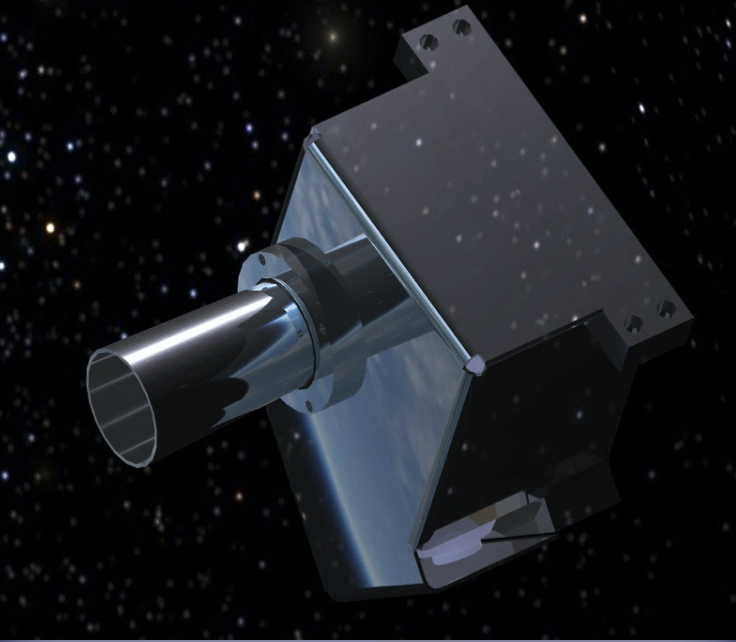
\includegraphics[width=0.49\textwidth]{fig/a.png}
    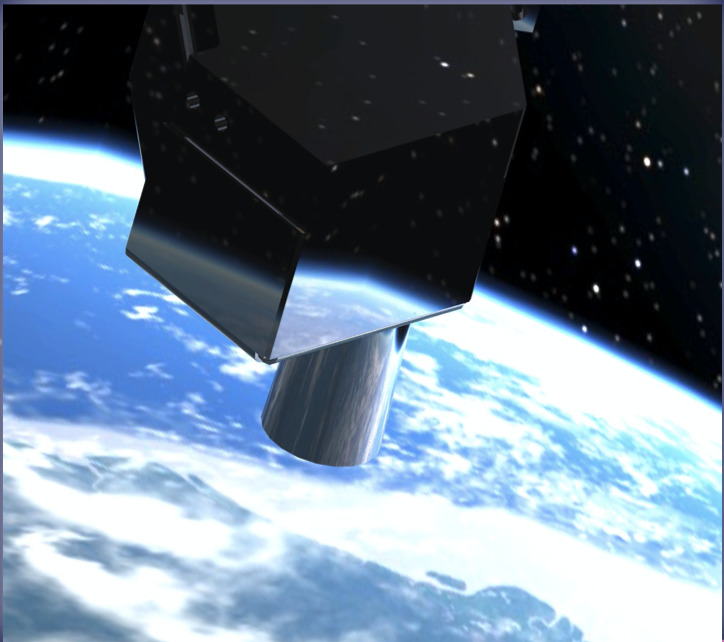
\includegraphics[width=0.49\textwidth]{fig/b.png}
    \caption{Renders del diseño preliminar del m\'odulo en el espacio}
    \label{fig:a}
\end{figure}
\begin{figure}[h!]
    \centering
    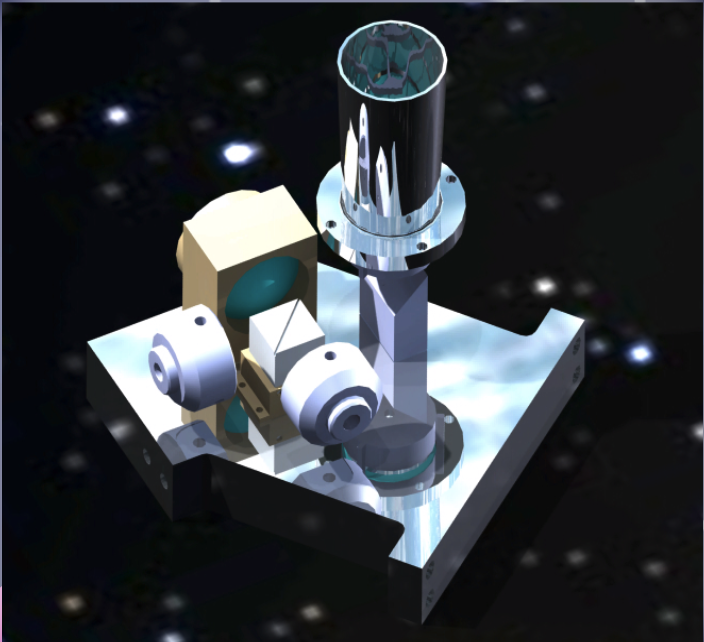
\includegraphics[width=0.55\textwidth]{fig/c.png}
    \caption{Render mostrando componentes}
    \label{fig:a}
\end{figure}
\newpage


\section{Análisis de costos y viabilidad}

En la presente sección se detallará el análisis de costos y la viabilidad económica del proyecto hasta el grado de ejecución alcanzado.\par

El presente análisis se concentrará en el estudio de los componentes necesarios para el diseño de nuestro \textit{Proof of concept} de FTIR.
\\\par
Los principales componentes necesarios para el módulo se pueden desglosar en cuatro categorías principales: óptica, electrónica, estructura y actuador. A continuación se detallan los mismos.
Dentro de la parte óptica, se puede encontrar un 
\begin{itemize}
    \item Corner cube mirror (2x US\$ 229)
    \item Mirrors \& Lenses (US\$ 200)
    \item Beam Splitter (US\$ 350)
\end{itemize}\par

Para la parte electrónica, se encuentra un
\begin{itemize}
    \item Ingaas Photodiode (US\$ 200)
\end{itemize}\par

En la sección de estructura, se tiene
\begin{itemize}
    \item Bulonería (US\$ 50)
    \item Material (US\$ 200)
\end{itemize}\par
Finalmente, en la parte de actuador, se encuentra:
\begin{itemize}
    \item Actuador lineal (US\$ 1250)
\end{itemize}

Al sumar estos costos parciales, se obtiene un total de US\$ 2708. Si bien este precio excede el
pensando inicialmente, se debe tener en cuenta la alta complejidad tanto técnica como teórica de la propuesta planteada, así como también el hecho de que al tratarse de un espectrómetro, la precisión de los componentes es indispensable para el correcto funcionamiento del dispositivo y tener una medición efectiva.
\\\par
Se puede observar el elevado precio del actuador lineal, ya que el mismo es una pieza fundamental del espectrómetro. Es él encargado de mover al espejo móvil en pasos del orden de los nanómetros, lo cual, en caso de fallar, afecta la relación rango- precisión. Teniendo estos factores en cuenta, se busco un actuador lineal que cumple con las características de precisión requeridas así como también tener la garantía del fabricante de que es un dispositivo \textit{Vacuum ready}. Por otro lado, el sensor, en este caso un fotodiodo, debe ser sensible en el rango de las longitudes de onda de interés y es imprescindible que tenga un bajo ruido para garantizar el funcionamiento del dispositivo. Por los motivos expresados anteriormente, resulta evidente que algunos componentes presenten elevados precios, ya que son necesarios para el correcto funcionamiento del módulo.


\section{Conclusión}

Ampliar el conocimiento acerca del ciclo del carbono y del impacto que tiene sobre la composición atmosférica se ha convertido en una necesidad no solo científica, sino también social. Hoy en día se pueden estimar flujos de estos gases a nivel continental, pero resultaría de extrema utilidad poder obtener información sobre sus concentraciones presentes en zonas específicas del planeta. Es decir, para lograr este cometido, se necesita mayor precisión y nuestra propuesta permitiría obtenerla empleando espectrómetros con un costo considerablemente inferior comparado a los que están actualmente en órbita en otras misiones espaciales.\par

\section{Comentarios Finales}

La medición de gases de efecto invernadero en la atmósfera mediante un satélite en órbita resulta un problema de gran complejidad, tanto del punto de vista óptico, como técnico. En comparación a otros temas o proyectos, la bibliografía disponible es escasa y con un alto nivel de complejidad técnico. Para la realización de este trabajo, los autores debieron realizar una investigación exhaustiva, leyendo bibliografía especializada y contactando a personalidades de la industria de distintas agencias espaciales. Dicha investigación permitió entender los conceptos detrás del principio de medición y los instrumentos utilizados para una misión de estas características.\par
Sin embargo, los autores creen que la única manera de inspirar y preparar una generación de jóvenes para participar en una nueva revolución espacial sólo es posible abordando desafíos complejos donde los jóvenes tendrán que utilizar sus conocimientos y sus capacidades críticas para la resolución de proyectos. Es importante destacar que se busca inspirar a jóvenes interesados en la industria aeroespacial a que pongan en práctica sus conocimientos, así cómo también se busca fomentar el aprendizaje en esta área, bajo la filosofía de que por más que se trate de conocimientos complejos, cualquiera que se disponga a aprenderlos, puede hacerlo. 



\newpage

\bibliography{biblio} 
% \bibliographystyle{ieeetr}
% \bibliographystyle{natbib}
\newpage



\section{Anexo}
\subsection[Teoría de transferencia radiativa]{Transferencia radiativa -- Para entender la radiometría}
\label{sec:teoria_radiometria}
El estudio de cuerpos reales (quasi-negros) en la radiometría parte del principio de la radiancia. Todo cuerpo emite fotones de varias longitudes de onda en función de su \textbf{\emph{temperatura}}. Los fenómenos que influyen en la medición de estos fotones son:
\begin{itemize}
    \item El \textbf{medio} que atraviesa el fotón. En el caso de satélites, dicho medio viene a ser la atmósfera. Este puede afectar en las siguientes formas:
    \begin{description}
        \item[Absorbancia:] El medio puede absorber los fotones incidentes causando un decremento en la intensidad medida. Este efecto depende de la longitud de onda, $\lambda$.
        \item[Dispersión:] Los fotones interactúan con el medio y son dispersados. Este efecto tambi\'en depende del $\lambda$ del fotón incidente. Las pérdidas por absorción y dispersión suelen llamarse \textit{extinción}.
        \item[Emisión:] Radiación emitida por el mismo medio. En mediciones desde satélites se tiene que considerar este efecto actuando sobre la Tierra (cuerpo que se desea medir), y sobre el satélite mismo ya que parte de los fotones que se miden son provenientes de la misma atmósfera.
    \end{description}
    \item La \textbf{temperatura} del cuerpo que se desea medir.
    \item La \textbf{dispersión del cuerpo} que se desea medir (causado por la emisión del medio en caso de haberlo).
    \item La \textbf{longitud de onda} $\lambda$ de los fotones que atraviesan el medio, si es que existe.
    \item Las especificaciones y \textbf{temperatura} de la antena: La antena no mide en un cono perfecto. Puede tener \textbf{"sidelobes"} que dependen de su eficiencia. La temperatura de la antena puede interferir.
\end{itemize}

Es importante destacar que un radiómetro no mide más que la potencia incidente para el rango de $\lambda$ que fue calibrado, el cual \textit{es un valor}, \textbf{\emph{escalar}}. Esto puede ser remediado agregando más radiómetros para formar un \textit{"phased-array"} o agregando un sistema mecánico de oscilación para recorrer un área con varias mediciones. 

La cantidad de mediciones que se pueden efectuar están limitadas por el ruido. Debido a esto es recomendable hacer un promedio temporal de mediciones para obtener el valor de la medición final. Esto se muestra en la ecuaci\'on \eqref{eq:EstimationByTemporalAvgRadiometer} (el sombrero de $\hat{P}_s$ indica promedio temporal).

\begin{equation} \label{eq:EstimationByTemporalAvgRadiometer}
    \hat{P}_s = \frac{1}{\tau} \int_\tau |s(t)|^2 ~\d t
\end{equation}
donde \(s\) es la señal medida. La ecuaci\'on \eqref{eq:EstimationByTemporalAvgRadiometer} tambi\'en es conocida como \textit{signal averaging}.

Considerando la extinción y la emisión del medio se llega a la ecuación de transferencia radiativa para un medio:
\begin{equation}
    \frac{\d T_B}{\d x} + \kappa_e \cdot T_B = \kappa_a T + \kappa_s T_{vs}
\end{equation}

\begin{description}
    \item[\(T_B\)]: Temperatura equivalente del fotón que atraviesa el medio estudiado
    \item[\(\kappa_a,\kappa_s \)]: Absorción y dispersión
    \item[\(T_{vs}\)]: Temperatura equivalente de la dispersión de volumen (ocasionada por nubes/lluvia)
    \item[\(T\)]: Temperatura física del medio
\end{description}

Lo que se termina midiendo en la antena es el fotón una vez que el mismo atraviesa el medio, a una distancia $x_{\sat}$.


\begin{equation}
   \boxed{ T_B(x_\sat) = T_B(0) \cdot \exp \left( -\int_0^{x_\sat} \kappa_e \d x \right) + \\ \int_0^{x_\sat} (\kappa_e T(x) + \kappa_s T_{vs}(x))\cdot \exp\left( -\int_x^{x_\sat}\kappa_e \d x_2\right) \d x }
\end{equation}

donde $x_2$ es una variable auxiliar.

La temperatura medida, $T_B(x_{\sat})$, se puede considerar directamente proporcional a la potencia para longitudes de onda cercanas a las microondas.


\subsection[Medición de indicadores]{Potencial técnica para la medición de gases invernaderos}

% 
Los satélites que observan la tierra miden la luz emitida y reflejada por la tierra y atmósfera. La luz reflejada presenta variaciones espectrales que reflejan la interacción de la radiación con las partículas. Para muchas frecuencias, la atmósfera es transparente a la radiación. Sin embargo, las longitudes de onda que excitan modos de vibración de las partículas gaseosas, son absorbidas por las mismas (haciéndolas vibrar en dicho modo). Por lo que la medición de la radiancia % Radiancia es la palabra correcta
es proporcional a la cantidad de partículas absorbentes presentes en la atmósfera. En dicho caso, la radiación proveniente de la tierra que llega al satélite sería igual a (aproximación de primer orden, Ref. \cite{spaceborn_sensing}):
\begin{equation}
    I(\lambda)=E_{0}(\lambda) R(\lambda) T(\lambda)
\end{equation}
Donde $E_{0}(\lambda)$ es la irradiancia de la parte más alta de la atmósfera, $R(\lambda)$ es la reflectancia de la superficie y $ T(\lambda)$ es la transmitancia atmosférica. $R(\lambda)$ presenta una variación muy suave con respecto a la longitud de onda y para un rango acotado de frecuencias se puede aproximar como constante o como función lineal de la longitud de onda. De forma similar, la irradiancia $E_{0}(\lambda)$ varía poco con respecto a la longitud de onda, excepto por algunas longitudes de onda bien identificadas, llamadas líneas de Fraunhoffer. Por otro lado, la transmitancia atmosférica $T(\lambda)$ muestra rápidos cambios espectrales, resultado de la suma de muchas líneas de absorción individuales de cada componente atmosférico. La amplitud de dichos picos está directamente relacionada con la cantidad del componente absorbente (de dicha longitud de onda).\par
%Ojo que temperatura y composición vertical también impacta la absorción.
Entonces, por medio de un instrumento de medici\'on de radiación (los mismos se evalúan en la sección \nameref{sec:instrumentos})  el cual mida longitudes de onda y radiancia de la misma, sería posible identificar las longitudes de absorción de varios gases  y deducir su concentración por medio de la radiancia de dicha longitud de onda. Al ser la absorción función de la presión atmosférica, se estaría midiendo un promedio de composición de gases a lo largo de la columna de atmósfera analizada. En caso de seguir desarrollando el concepto y de que la resolución del instrumento elegido lo permita, se podría mejorar el modelo dándole más peso a las capas atmosféricas más bajas (Dufour and Breon, 2003).\par 




 \subsection{Figuras}\label{subsec:figuras}
\begin{figure}[htb!]
	\centering
	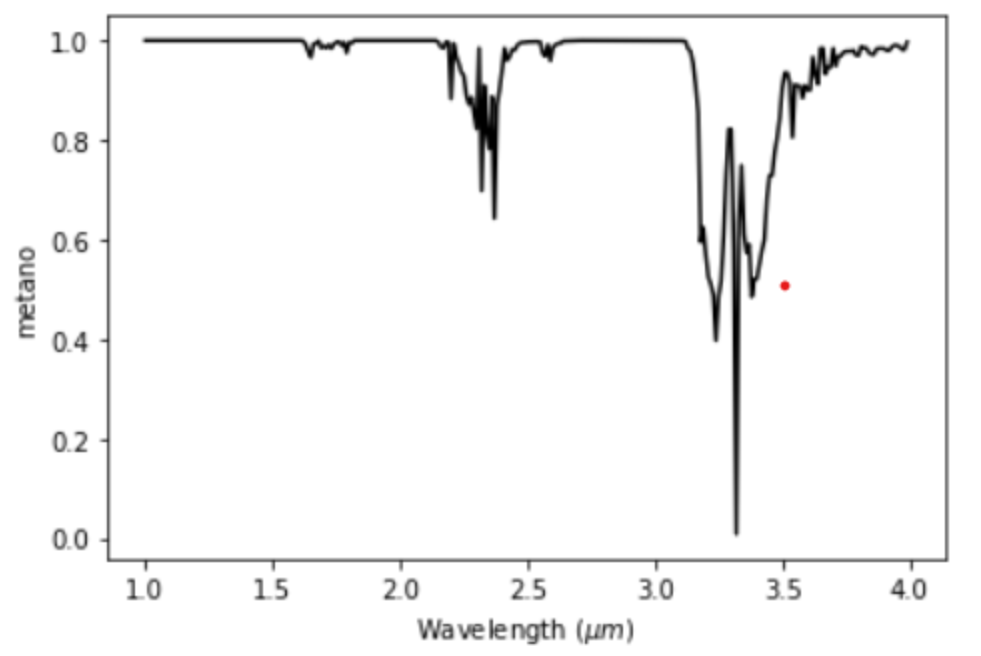
\includegraphics[width=10cm]{fig/absorbmetano.png}
	\caption{Absorción del metano Vs longitud de onda}
	\label{fig:absorbMetano}
\end{figure}

\begin{figure}[htb!]
	\centering
	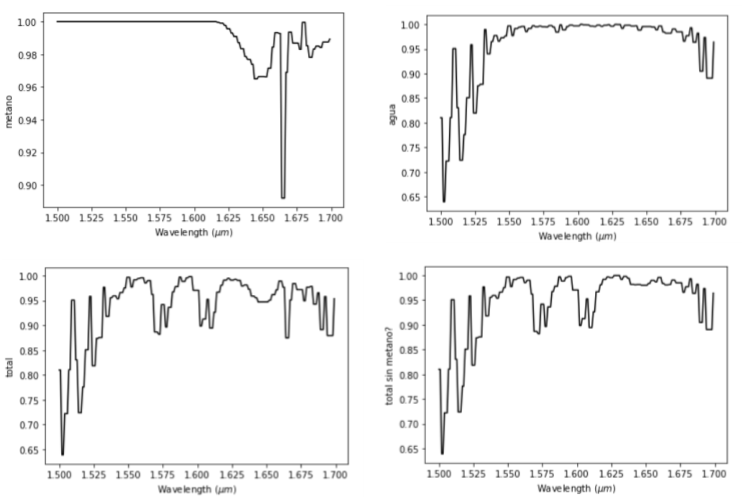
\includegraphics[width=15cm]{fig/analisis16.png}
	\caption{Análisis a 1.6 µm}
	\label{fig:analisis16}
\end{figure}

\begin{figure}[htb!]
	\centering
	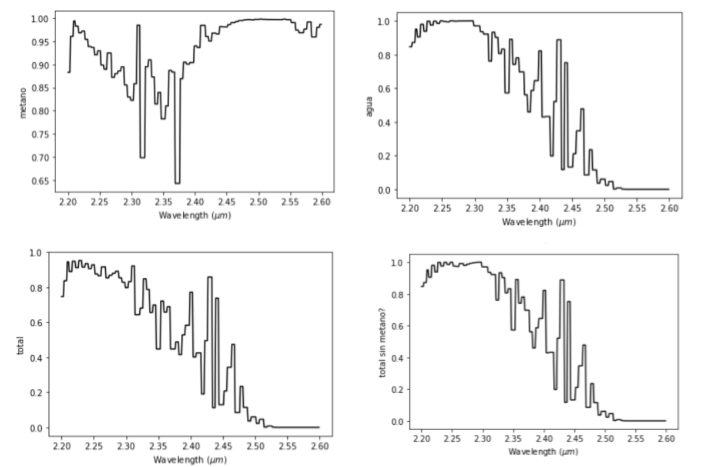
\includegraphics[width=15cm]{fig/analisis24.png}
	\caption{Análisis a 2.4 µm}
	\label{fig:analisis24}
\end{figure}
\begin{figure}[htb!]
	\centering
	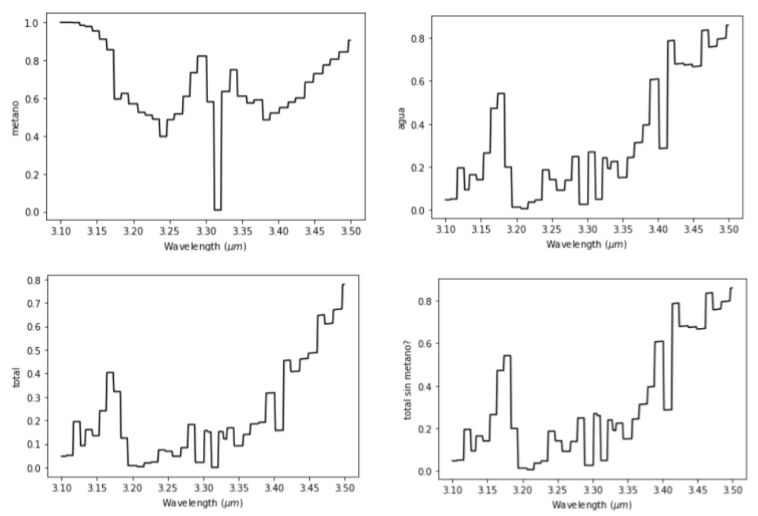
\includegraphics[width=15cm]{fig/analisis33.png}
	\caption{Análisis a 3.3 µm}
	\label{fig:analisis33}
\end{figure}

\newpage
\subsection{Código de simulaciones}

\begin{lstlisting}[language=Python, caption=Python example]
import matplotlib.pyplot as plt
import numpy as np
import scipy.signal as ss
import scipy as scipy
import matplotlib as mpl
import math
import pandas as pd
from scipy.interpolate import interp1d

from google.colab import files
uploaded = files.upload()

pd.set_option("display.max_rows", None, "display.max_columns", None)
print(df1)
df1.plot(kind='line', x='wl', y='I_R')
df2.plot(kind='line', x='wl', y='I_R')

#Caracteristicas instrumento
x_step = 99e-9 #En m
N = 1000 #Cantidad de samples
lmin_sensor = 400e-9
lmax_sensor = 2500e-9

#Entonces el instrumento tiene: (#d: optical. x:x)
x_range = (N - 1) * x_step
d_step = 2 * x_step 
d_range = 2 * x_range

print('Características Instrumento:')
print('paso x (nm):',x_step*1e9)
print('paso d (nm):',d_step*1e9)
print('distancia (cm):',x_range*1e2)
print('dco (cm):',d_range*1e2)
print('Minima longitud de onda posible (um):',(2*d_step)*1e6)
print('Maximo número de onda posible (cm$^-1$)',1/(2*d_step)*1e-2)

#Caracteristicas input simulación
input_domain_units = 1e-6  #[m], Dominio de entrada en um, data en I/m^2/[um]
N_data = len(np.array(df1['wl']))
lambda_min = df1.at[0, 'wl'] * input_domain_units
lambda_max = df1.at[N_data-1, 'wl'] * input_domain_units
delta_lambda = (df1.at[1, 'wl']-df1.at[0, 'wl']) * input_domain_units
v_max = 1/lambda_min
v_min = 1/lambda_max
print('Data de Entrada:')
print('lambda_min (um):', lambda_min*1e6)
print('lambda_max (um):', lambda_max*1e6)
print('v_max (cm$^{-1}$):', v_max*1e-2)
print('v_min (cm$^{-1}$):', v_min*1e-2)
plt.figure(1)
plt.plot(np.array(df1['wl']),np.array(df1['I_R']))
plt.title('Data de entrada')
plt.xlabel('Longitud de Onda (um)')
plt.ylabel('W/m$^2$/um')

#Características output simulación
output_domain_units = 100 #[m^-1], Dominio de salida en cm^-1, data en W/m^2/[cm^-1]

#Zero Padding en numero de onda para que quede interpolado en d para sampling k*d_step para algun valor de k
k_os_min = 1+int(np.floor(2*d_step*v_max)) #oversampling #ROUND INTEGER TO NEXT INTEGER
print('Oversampling a utilizar:', k_os_min)
v_os = (1/d_step)*k_os_min
v_spec_max = v_os/2 #Frecuencia maxima en el espectro
N2 = int(np.ceil(1+v_spec_max*lambda_max**2/delta_lambda)) #N Calculado con criterio de conservar resolución minima

#Paso en frecuencia
delta_v = v_spec_max / N2 
#Redondear data a bines
v_min = np.ceil(v_min / delta_v) * delta_v  #Redondear v_min a un bin
v_max = np.floor(v_max / delta_v) * delta_v  #Redondear v_max a un bin
#Generar vector de v equiespaciado v_int (numeros enteros, indica múltiplos de delta_v)
v_int = np.linspace(int(v_min/delta_v),int(v_max/delta_v),(int((v_max-v_min)/delta_v)+1))
#(precisión numérica)
v_int = [int(i) for i in np.round(v_int)]

#Entonces
print('N2 (Espectro generado): ', N2)
print('v_min (redondeado a bin, cm$^{-1}$): ', v_min*1e-2)
print('v_max (redondeado a bin, cm$^{-1}$): ', v_max*1e-2)
print('delta_v (paso en número de onda, cm$^{-1}$): ', delta_v*1e-2)

#Calcular longitudes de onda asociadas a numeros de onda para interpolar, en unidades de entrada
v_dom_interp = [ delta_v * i/output_domain_units for i in v_int]  # En unidades de salida
#l_dom_interp = [ 1e4/i for i in v_dom_interp]
l_dom_interp = [1/(input_domain_units*output_domain_units)/i for i in v_dom_interp] #En unidades de entrada
l_original_domain = np.array(df1['wl'])
I_original_data = np.array(df1['I_R'])
#Recortar espectro
I_sensor_data = [0 if (l_original_domain[i]*input_domain_units < lmin_sensor or l_original_domain[i]*input_domain_units > lmax_sensor) else I_original_data[i] for i in range(len(I_original_data))]
I_interp_data_f = interp1d(l_original_domain, I_sensor_data, kind='slinear',fill_value=[0])
I_interp_data = I_interp_data_f(l_dom_interp) #Esta seria la funcion I_data_lambda(1/v)
#Aplicar jacobiano (1/v^2)
#I_v = 1e4 * np.divide(I_interp_data,v_dom_interp)
I_v = 1/(input_domain_units*output_domain_units) * np.divide(I_interp_data,v_dom_interp)
I_v = np.divide(I_v,v_dom_interp)

#Espectro de partida
I = np.zeros(N2)
I[v_int] = I_v
plt.figure(2)
plt.plot(I)
plt.title('Espectro generado a partir de data')
plt.xlabel('bin')
plt.ylabel('W/m$^2$/cm$^{-1}$')

#Antitransformar para obtener interferograma de partida
dv = delta_v/output_domain_units  #Diferenciales en output_domain_units, al integrar W/m^2/cm^-1*cm^-1 = W/m^2
I_d = np.fft.irfft(I)*len(I)*dv
print('I_d : ', I_d)
print('i_d length', len(I_d))

#En base al interferograma obtenido, se calculará interferograma simulado
nuevo_id = np.zeros(2 * N)
#VENTANA A UTILIZAR
window = ss.windows.get_window('blackmanharris',2*N)
window2 = np.zeros(2*N)
for i in range(N):
  window2[i] = window[N-1+i+1]
  window2[N-1+i+1] = window[i]
for i in range(int(len(nuevo_id)/2)):
  if i < N2/2:
    nuevo_id[i] = I_d[k_os_min*i]
    nuevo_id[2*N - i - 1] = I_d[k_os_min*(1+i)]
  else:
    #Se utilizaron todos los datos
    #zero padding interpolará valores en frecuencia
    nuevo_id[i] = 0
    nuevo_id[2*N - i - 1] = 0
# APLICAR VENTANA
interferogram_record = np.array(nuevo_id)
interferogram_record = interferogram_record + interferogram_record[0]
for i in range(2*N):
  nuevo_id[i] = nuevo_id[i] * window2[i]

#Interferograma Original
plt.figure(3)
plt.plot([i*d_step/k_os_min*1e2 for i in range(int(len(I_d)/2))],[I_d[i]*1e3 for i in range(int(len(I_d)/2))])
plt.title('Interferograma generado a partir de data')
plt.xlabel('dco [cm]')
plt.ylabel('mW/m$^2$')

#Nuevo Interferograma
plt.figure(5)
plt.plot([i*d_step*1e2 for i in range(N)],[nuevo_id[i]*1e3 for i in range(N)])
plt.title('Interferograma ventaneado y resampleado')
plt.xlabel('dco [cm]')
plt.ylabel('mW/m$^2$')



#Obtener espectro
dd = d_step
spec = 2*np.absolute(np.fft.rfft(nuevo_id))*dd #TODO: XQ TENGO QUE MULTIPLICAR POR DOS?
#Al integrar, W/m^2*m = W/m^2/m, se busca W/m^2/(output_domain_units)
spec = spec*output_domain_units #Al transformar queda en W/m^2/(m^-1), convertir en W/m^2/(output_domain_units)

v_int_espectro_nuevo = np.linspace(0,len(spec)-1,len(spec))/len(spec)
v_int_espectro_original = np.linspace(0,len(I)-1,len(I))/len(I)

#graficar los dos juntos
plt.figure(6)
plt.plot(v_int_espectro_original*(k_os_min/(d_step*2))*1e-2,I)
plt.title('Espectro Original')
plt.xlabel('número de onda (cm$^{-1}$)')
plt.ylabel('W/m$^2$/cm$^{-1}$')
plt.figure(7)
plt.plot(v_int_espectro_nuevo*(1/(d_step*2))*1e-2,spec)
plt.title('Espectro Obtenido')
plt.xlabel('número de onda (cm$^{-1}$)')
plt.ylabel('W/m$^2$/cm$^{-1}$')
plt.figure(8)
plt.plot(v_int_espectro_original*(k_os_min/(d_step*2))*1e-2,I)
plt.plot(v_int_espectro_nuevo*(1/(d_step*2))*1e-2,spec)
plt.title('Espectros Superpuestos')
plt.xlabel('número de onda (cm$^{-1}$)')
plt.ylabel('W/m$^2$/cm$^{-1}$')
plt.figure(9)
plt.plot(v_int_espectro_original*(k_os_min/(d_step*2))*1e-2,I) #cm^-1
plt.plot(v_int_espectro_nuevo*(1/(d_step*2))*1e-2,spec) #cm^-1
plt.xlim([1e-2/lmax_sensor,1e-2/lmin_sensor])
plt.title('Espectros Superpuestos, recortado')
plt.xlabel('número de onda (cm$^{-1}$)')
plt.ylabel('W/m$^2$/cm$^{-1}$')

plt.figure(10)
plt.plot(v_int_espectro_nuevo*(1/(d_step*2))*1e-2,spec) #cm^-1
plt.xlim([1e-2/lmax_sensor,1e-2/lmin_sensor])
plt.title('Espectros Obtenido, recortado')
plt.xlabel('número de onda (cm$^{-1}$)')
plt.ylabel('W/m$^2$/cm$^{-1}$')

#Graficar ventana utilizada
plt.figure(11)
plt.plot(window)
plt.plot(window2)
plt.title('Ventana utilizada')
plt.xlabel('Dominio (cm)')
plt.ylabel('K')

#Interferogram Record
plt.figure(12)
plt.plot([i*d_step*1e2 for i in range(N)],[interferogram_record[i]*1e3 for i in range(N)])
plt.title('Interferogram Record')
plt.xlabel('dco [cm]')
plt.ylabel('mW/m$^2$')

\end{lstlisting}
%The differential absorption technique requires clear sky
%along the line of sight. It also requires sunlight with a sun
%sufficiently high above the horizon to limit scattering in
%the atmosphere. These requirements limit the time-space
%sampling capabilities. In particular, no night measurement
%is possible, and high latitudes are not sampled during the
%winter season. This is a limitation to quantify processes
%such as winter ecosystem respiration, or CH4 emissions by
%boreal and arctic regions. Another constraint is that the
%surface reflectance must be large enough as it has a direct
%impact on the signal-to-noise. Over land, natural surfaces
%are relatively dark at the wavelengths of interest, in
%particular when they are snow-covered. However, the
%problem is mostly over water that is extremely dark, and
%therefore not suitable for the measuring technique, except
%in the direction of the glint. As a consequence, measurements over the oceans are only possible when the
%instrument aims at the sun glint, which limits the spatial
%coverage and puts some constraints on the instrument
%design.


%\input{apunte.tex}

\end{document}